\documentclass[letterpaper,10pt]{article}
\usepackage[dvips]{graphicx}
\usepackage{mathrsfs}
\usepackage{graphics}
\usepackage{fullpage}
\usepackage{latexsym}
\usepackage{amsmath}
\usepackage{amssymb}
\usepackage{pstricks, egameps, sgame}
\usepackage{bbm}
\usepackage{multirow}
\usepackage{pgfplots}

\begin{document}
\author{Desmond C. Ong, Emily Yeh}
\title{Machine Learning Summary Notes}
\date{Autumn 2012}
\maketitle
\textit{This set of notes are compiled from my and the instructors' lecture notes taken during Stanford's CS 229 Machine Learning course, as well as the free online offering at Coursera, both taught by Andrew Ng. This set of notes will be divided into two parts: the first part will contain summaries of various ML techniques designed to serve as quick primers and reference material, while the second part will contain more theory.}

\tableofcontents

\newpage

\begin{table}[hbtp]
\center
\begin{tabular}{c|c|c|c}
Type & Name & Output/Use & Blah \\
\hline
\multirow{4}{*}{Supervised} & Linear Regression & Continuous Variable & \\
& Logistic Regression & Classifier & \\
& Neural Networks & Classifier (non-linear) & \\
& Support Vector Machines & Classifier (non-linear) & \\
\hline
\multirow{5}{*}{Unsupervised} & K-means Clustering & Classifier & \\
& Mixture of Gaussians  & & \\
& Factor Analysis & & \\
& Principal Component Analysis & & \\
& Independent Component Analysis  & & \\
\hline
& Reinforcement & & \\
\end{tabular}
\caption{Comparison between ML Techniques} \label{SummaryTable}
\end{table}


Choosing which unsupervised learning algorithm to use along two dimensions: What kind of structure do you expect your data to have, and the type of algorithm used.

\begin{table}[hbtp]
\center
\begin{tabular}{c|c|c}
Data likely resides in ... \textit{(structure of data)} /  & Model P(x) (density estimation) & Non-probabilistic model \\
Type of model \textit{(purpose)} & \textit{(Anomaly Detection)} & \textit{(Compression, visualization)} \\
\hline
 a lower-dimensional subspace? & \multirow{2}{*}{Factor Analysis} & \multirow{2}{*}{Principal Component Analysis} \\
\textit{($n>m$ ok)} & & \\
 \hline
clumps or clusters in $n$ dimensions? & \multirow{2}{*}{Mixture of Gaussians} & \multirow{2}{*}{k-means clustering} \\
\textit{($n<m$)} & & \\
\end{tabular}
\caption{Choosing Unsupervised Learning Algorithms} \label{UnsupervisedSummary}
\end{table}


\section{Introduction}

In this digital age, we are inundated with huge data sets that we need to make sense of. One of the ways to solve these problems involve using automated techniques that require computers to learn to make sense from the data sets. Enter Machine Learning.

Machine Learning is widely used everywhere, including but not limited to: Spam filters; Google searches and Web page ranking; friend recognition on Facebook; computational biology; data mining; autonomous helicopter flying; handwriting recognition; Natural Language Processing; Computer Vision.

Two brief definitions of Machine Learning:
\begin{quote}
Field of study that gives computers the ability to learn without being explicitly programmed.\\
Arthur Samuel (1959)
\end{quote}

\begin{quote}
Well-posed learning problem: A computer program is said to learn from experience \textbf{E} with respect to some task \textbf{T} and some performance measure \textbf{P}, if its performance on \textbf{T}, as measured by \textbf{P}, improves with experience \textbf{E}. \\
Tom Mitchell (1998) 
\end{quote}

There are several different types of Machine Learning. There are three main types that will be covered in these notes: \textit{Supervised Learning}; \textit{Unsupervised Learning}; and \textit{Reinforcement Learning}.

Supervised learning requires a data set of labels, or ``right answers", often called the \textit{training set}. Example problems include \textit{classification} problems, which aim to output classifications or groupings (``What will the weather be like tomorrow?"); and \textit{regression} problems, which aim to output a continuous variable (``What will the temperature be tomorrow?")

Unsupervised learning, on the other hand, does not require a labelled data set. The aim of unsupervised learning is to find structure in the data. Such algorithms include \textit{clustering} algorithms, which groups data into ``clusters" where points within a cluster share some similarity with each other.

Reinforcement learning involves \ldots


\section{Supervised Learning: (Multiple) Linear Regression}

\subsection{Gradient Descent}
Linear regression can be used in problems where your desired output is a continuous-valued variable. Some definitions are provided in a footnote\footnote{Definitions:
\begin{itemize}
	\item $m \equiv$ number of training examples
	\item $x \equiv$ ``input" variables, or features
	\item $y \equiv$ ``output" variable, or ``target" variable
	\item $(x^{(i)},y^{(i)}) \equiv$ $i$-th training sample ($i \leq m$)
	\item $n \equiv$ number of features
	\item $x_j \equiv$ $j$-th feature ($j \leq n$, but remember to include $x_0$)
	\item $\theta \equiv$ regression parameters
	\item $h \equiv$ hypothesis, (a mapping from $x$ to $y$). E.g. $h_\theta (x) = h(x)= \theta_0 + \theta_1 x + \ldots$
	\item Note that $x_0 = 1$ (So that we can have $h_\theta (x) = \vec \theta^T x = \theta_0 x_0 + \theta_1 x_1 + \ldots $)
	\item $J \equiv$ cost function to minimize. Regression is to minimize $J(\vec \theta) = \frac{1}{2m} \sum_{\forall i} \left( h_{\vec \theta} (x^{(i)}) - y^{(i)} \right)^2$
\end{itemize}
}. The basic problem is, given a training set $(x,y)$, where $x=(x_1,\ldots,x_j)$ is a vector, and represents our $(j)$ input variables (independent variables) and $y$ represents our output variable (dependent variable). We want to predict new $y$s given new $x$s.

For example, let's say for some $x$ we are trying to solve for $y$. We have the following dataset of $x$ values and corresponding $y$ results (see Figure 2.1). In order to find the optimal model for this data, we want to predict the cost for prediction models and find the model with the least cost.
%%FIGURE 2.1
\begin{figure}
\centering
\begin{tikzpicture}
\begin{axis}[%
scatter/classes={%
    a={mark=o,draw=black}}]
\addplot[scatter,only marks,%
    scatter src=explicit symbolic]%
table[meta=label] {
x y label
1 2 a
2 1.5 a
3 2.7 a
4 2.3 a
5 3.2 a
6 5.4 a
7 7.2 a
8 7.7 a
9 4.8 a
10 9.2 a
11 7.5 a
12 6.8 a
    };
%\addplot[mark=none, color=red] coordinates{
%(0, 0.1)
%(10, 8)
%};
\end{axis}
\end{tikzpicture}
\begin{tikzpicture}
\begin{axis}[%
scatter/classes={%
    a={mark=o,draw=black}}]
\addplot[scatter,only marks,%
    scatter src=explicit symbolic]%
table[meta=label] {
x y label
1 2 a
2 1.5 a
3 2.7 a
4 2.3 a
5 3.2 a
6 5.4 a
7 7.2 a
8 7.7 a
9 4.8 a
10 9.2 a
11 7.5 a
12 6.8 a
    };
\addplot[mark=none, color=red] coordinates{
(0, 0.1)
(10, 8)
};
\end{axis}
\end{tikzpicture}\\
{\bf Figure 2.1. (Left) Sample dataset for a regression supervised learning problem. (Right) Sample dataset with prediction model in red.} 
\end{figure}

We do this by first forming a hypothesis for our prediction model. The hypothesis (regression equation) links the predicted value of $y$ to the independent variables $x$. The \textit{Gradient Descent} method tries to minimize the gradient of the error of this hypothesis. (For those familiar with regressions, this is the ordinary least squares model).

\begin{align}
\text{Hypothesis: }& h_\theta (x) = \theta_0 + \sum_{j=1}^n \theta_j x_j = \theta^T x\\
\text{Gradient = derivative of }(h-y)\text{: }& J(\theta)=\frac{1}{2} \sum_{i=1}^m \left( h_{\theta}(x^{(i)}) - y^{(i)}  \right)^2 \\
\text{Least Means Squares Update Rule: }& \theta_j := \theta_j - \alpha \frac{\partial}{\partial \theta_j} J(\vec \theta) \label{EqnLMS} \\
&\quad = \theta_j - \alpha \frac{1}{m} \sum_{i=1}^m \left( h_{\theta}(x^{(i)}) - y^{(i)}  \right) x_j^{(i)} \notag
\end{align}

One way you could visualize this is that the graph of $J$ against $\theta$ would look like a convex, or ``bowl" shaped function, and we wish to minimize the value of $J$ with respect to $\theta$, i.e. we want to find the minimum of the bowl (see Figure 2.2). The $\alpha$ in Eqn. \ref{EqnLMS} is called the learning rate. If the learning rate is too small, the convergence for gradient descent will be too slow. On the other hand, if the learning rate is too large, then each iteration of gradient descent might overshoot the minimum, eventually failing to converge, or even diverging. Note that as the gradient descent algorithm approaches a local minimum, the second term in the update equation will automatically be smaller and hence gradient descent will automatically take smaller steps, so there is no need to decrease $\alpha$ over time.
\begin{figure} %FIGURE 2.2
\centering
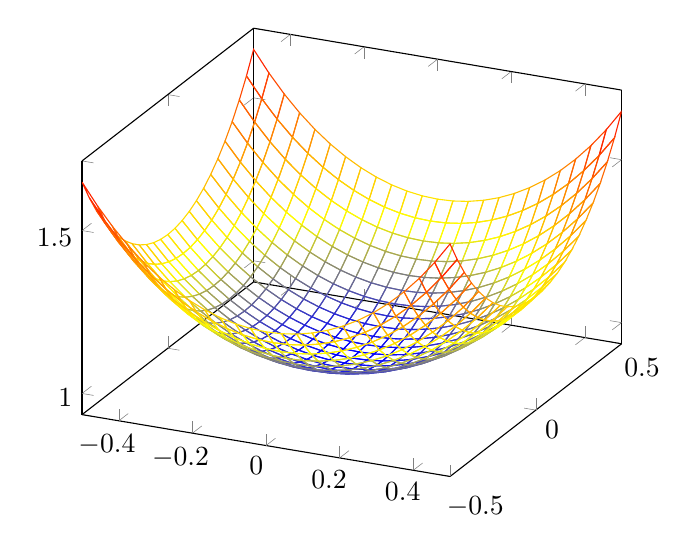
\begin{tikzpicture}
	\begin{axis}
	\addplot3[mesh,domain=-0.5:0.5] {exp(x^2+y^2)};	
	\end{axis}
\end{tikzpicture}\\
{\bf Figure 2.2. Plot of parameter values for cost function J($\theta_0$,$\theta_1$) on resulting cost.}
\end{figure}

\subsection{Gradient Descent Implementation}

A test for convergence is easily done by plotting $J(\theta)$ as a function of number of iterations, and declare convergence if $J(\theta)$ decreases by say, less than $10^{-3}$ in one iteration. (It might be helpful too to see the plot, to see whether the learning rate is appropriate, etc.)

One suggestion to choosing $\alpha$ is to vary $\alpha$ logarithmically in steps of 1/3. E.g. $\alpha = 0.01, 0.03, 0.1, 0.3, 1 \ldots$, and testing the convergence.

Note that when doing the updating in Eqn. \ref{EqnLMS}, all the $\theta$ parameters must be updated simultaneously. This makes sense because the second term in the update equation depends on all the rest of the $\theta$s, and once you update $\theta_i$ to $\theta_i'$, the update equation for $\theta_{j\neq i}$ will depend on (the new) $\theta_i'$ rather than (the old) $\theta_i$. (Doing the updating with vectorization automatically takes care of this). 

There are two ways to actually implement this algorithm. \textbf{Batch gradient descent} computes the update equation for the entire training set (i.e. all pairs of $x$ and $y$), and then updates the parameters $\theta$. \textbf{Stochastic gradient descent}, or incremental gradient descent, on the other hand, computes the update equation for one training example (i.e. one pair of $x$ and $y$) at a time and then updates $\theta$. (This is useful if data is coming in one at a time.)\\\\
{\bf Summary of Gradient Descent Method:}
	\begin{enumerate}
	\item Begin with some $\theta$
	\item Change until find minimum $J$
	\item $\theta_j := \theta_j - \alpha \frac{\partial}{\partial \theta_j} J(\vec \theta) = \theta_j - \alpha \frac{1}{m} \sum_{i=1}^m \left( h_{\theta}(x^{(i)}) - y^{(i)}  \right) x_j^{(i)}$
	\end{enumerate}
	\begin{itemize}
	\item Con: Need to choose an optimal $\alpha$ that won't overshoot or take too much time.
	\item Con: Needs many iterations.
	\item Pro: Works well even if $n$ is large ($10^6$)
	\end{itemize}
	
\subsection{Feature Scaling} The idea behind \textbf{feature scaling} is that the many variables $x$ might have vastly different scales. E.g. $x_1$ could be on the order of $10^6$ while $x_2$ could be on the order of $10^2$ in their respective units. In this case, the algorithm might take much longer to reach convergence. One way to achieve feature scaling is to normalize every feature to be within $-1\leq x_i \leq 1$ by subtracting each feature by its mean and dividing by its standard deviation.
\begin{equation}
\text{Feature scaling: }\quad x_i \rightarrow \frac{(x_i-\mu_i)}{\sigma_i}\label{EqnNormalization}
\end{equation}




\subsection{Normal Equation Method}

The Normal equation method is a way to solve for $\theta$ analytically, with no need for iteration and no need to choose $\alpha$ and scale features. However, this would be slow if $n$ is large, because we would need to compute the inverse\footnote{Extra: what if $\left( X^T X \right)$ is non-invertible? One possibility is that you have redundant (usually linearly dependent) features, and another possibility is that you have too many features $(m \leq n)$; delete some features, or use regularization.} of a $n\times n$ matrix: $\left( X^T X \right)^{-1} \sim O(n^3)$.

Given a training set, the design matrix $X$ is an $m \times (n+1)$ matrix (including the intercept term), where each row corresponds to one training example, and each column would correspond to a feature. Let $y$ be the $m (\times 1)$-dimensional vector corresponding to the target values. We define $\theta$ to be the $(1 \times) (n+1)$-dimensional parameter vector.

Given $h_\theta(x^{(i)}) = (x^{(i)})^T \theta$, the $m$ rows of $X \theta - y$ would be $[h_\theta(x^{(i)}) - y^{(i)}]$. Notice then that 
\begin{align}
J(\theta) = \frac{1}{2} || X\theta - y ||^2 = \frac{1}{2} (X\theta - y)^T (X\theta - y)
\end{align}
Taking the derivative:

\begin{align}
\nabla_\theta J(\theta) &= \nabla_\theta \frac{1}{2} (X\theta - y)^T (X\theta - y) \\
&=\frac{1}{2} \nabla_\theta  (\theta^TX^TX\theta - y^TX\theta  - \theta^TX^Ty + y^Ty ) \\
&=\frac{1}{2} \nabla_\theta  \text{tr}( \theta^TX^TX\theta - y^TX\theta  - \theta^TX^Ty) \quad ; \text{trace of a real number is itself / $\nabla_\theta y^Ty = 0$}\\
&=\frac{1}{2} \nabla_\theta  (\text{tr} \theta^TX^TX\theta - 2\text{tr}(y^TX\theta)) \quad ; \text{tr}A=\text{tr}A^T \\
&=\frac{1}{2} (X^TX\theta + X^TX\theta - 2X^Ty) \quad ; \nabla_A \text{tr}ABA^TC = B^TA^TC^T + BA^TC \\
&= X^TX\theta - X^Ty
\end{align}
Thus, setting the derivative to zero, we find that
\begin{align}
X^TX\theta = X^Ty \\
\theta = (X^TX)^{-1}X^Ty
\end{align}

\subsection{Probabilistic Interpretation}

%%%%%%%%%%%% ----- TODO ------ %%%%%%%%%%%%
(Incomplete)

\subsection{Locally weighted linear regression}

%%%%%%%%%%%% ----- TODO ------ %%%%%%%%%%%%
(Incomplete)
	

\section{Supervised Learning: Classification and Logistic Regression}
\begin{itemize}
\item Used to solve classification problems (desired output: classifier variable)
\item Linear regression not advised for classification. First, it is sensitive to outliers/skewed data sets
\item Logistic function (Sigmoid function): $g(z) = \frac{1}{1+e^{-z}}$
	
	\begin{itemize}
	\item Hypothesis: $h_{\theta}(x)$ = estimated probability that $y=1$ on input $x$, or $h_{\theta}(x) = P(y=1|x;\theta)$
	\item Predict $y=1$ if $h_{\theta}(x) \geq 0.5$, or since $h_{\theta}(x) = g(\theta^T x) \implies \theta^Tx \geq 0$
	\item Linear regression cost function cannot be used as $g(x)$ is non-linear and the cost function will be a non convex function.
	\item Thus, we use the following cost function:
	$$
	\text{Cost}\left( h_{\theta}(x),y \right) = \left\{
     	\begin{array}{lr}
       	-\log\left(h_{\theta}(x) \right) & \quad \text{if  } y=1\\
       	-\log\left( 1 - h_{\theta}(x) \right) & \quad \text{if  } y=0
     	\end{array}
   	\right.
	$$
	\item Intuition: if $y=1$, penalize more as $h_{\theta}(x) \rightarrow 0$, and if $y=0$, penalize more as $h_{\theta}(x) \rightarrow 1$
	\item Because $y$ can only take on values of $0$ or $1$, we can write:
	\item $\text{Cost}\left( h_{\theta}(x),y \right) = -y\log\left(h_{\theta}(x) \right) - (1-y)\log\left(1 - h_{\theta}(x) \right) $
	\item $J(\theta) = \frac{1}{m} \sum_{i=1}^m \text{Cost}\left( h_{\theta}(x^{(i)}),y^{(i)} \right) = -  \frac{1}{m} \sum_{i=1}^m \left[ y^{(i)}\log\left(h_{\theta}(x^{(i)}) \right) + (1-y^{(i)})\log\left(1 - h_{\theta}(x^{(i)}) \right) \right]$
	\item $\theta_j := \theta_j - \alpha \frac{\partial}{\partial \theta_j} J(\theta) = \theta_j - \alpha \frac{1}{m} \sum_{i=1}^m \left( h_{\theta}(x^{(i)}) - y^{(i)}  \right) x_j^{(i)}$
	\end{itemize}
\item Decision boundary ``separates" variable space into two decision regions. Can be linear or non-linear.

\item Advanced Optimization
	\begin{itemize}
	\item There are other optimization algorithms besides gradient descent.
	\item E.g. Conjugate gradient; BFGS; L-BFGS.
	\item Pros: No need to choose $\alpha$, and often faster than gradient descent.
	\item Cons: More complex.
	\end{itemize}
	
\item For multi-class classification,
	\begin{itemize}
	\item One-vs-all: For each class $i$, train a logistic regression classifier $h_\theta^{(i)}(x)$ to predict probability that $y=i$.
	\item On new input $x$, to make a prediction, pick $i$ that maximizes the classifier $h_\theta^{(i)}(x)$
	\end{itemize}
\end{itemize}


\section{Supervised Learning: Support Vector Machine}

(Abridged version from Coursera notes)

The optimization objective for SVMs is similar to logistic regression (classification), but with several key differences, especially in convention. 1) SVM does not normalize by the number of examples, $\frac{1}{m}$. This does not affect the $\theta$ that minimizes the cost function.

While regularized logistic regression looks like $A+\lambda B$, SVM uses $CA + B$, where setting $C$ to be small corresponds to setting $\lambda$ to be large.

SVM uses ``cost" terms instead of the log terms. Define:

cost$_1(\theta^Tx)$ is 0 for $\theta^Tx \geq 1$ and increases as $\theta^Tx$ decreases

cost$_0(\theta^Tx)$ is 0 for $\theta^Tx \leq -1$ and increases as $\theta^Tx$ increases

\begin{align}
\min_\theta C \sum_{i=1}^m \left[ y^{(i)} \text{cost}_1(\theta^Tx^{(i)}) + (1-y^{(i)})\text{cost}_0(\theta^Tx^{(i)}) \right] + \frac{1}{2}\sum_{j=1}^n \theta_j^2
\end{align}
Hypothesis:
\begin{align}
	h_\theta (x) =
     	\begin{cases}
       	1 & \text{if  } \theta^Tx \geq 0 \\
       	0 & \text{otherwise  }
     	\end{cases}
\end{align}

\subsection{Large Margin Intuition}
In order to minimize cost: if $y=1$, want $\theta^Tx \geq 1$ (not just $\geq 0$, which is sufficient for classification). Similarly, if $y=0$, want $\theta^Tx \leq -1$ (not just $< 0$). If C is very large, the problem becomes: 

\begin{align}
\min_\theta \frac{1}{2} \sum_{j=1}^n \theta_j^2  \\
\text{ s.t. } \theta^Tx^{(i)} \geq 1 \qquad \text{if  } y^{(i)}=1 \\
\theta^Tx^{(i)} \leq -1 \qquad \text{if } y^{(i)}=0
\end{align}

If we solve the problem with $C$ very large and the previous two constraints, we get a very robust decision boundary with a large margin. (Hence, SVM is called a large margin classifier)

\subsection{Mathematics Behind Large Margin Classification}
Thinking in terms of 2-norms, the problem becomes:
\begin{align}
\min_\theta \frac{1}{2} \vert \vert \theta \vert \vert ^2
\end{align}

Now, consider $\theta^Tx^{(i)} = p^{(i)} \cdot \vert \vert \theta \vert \vert = \theta_1 x_1^{(i)} \theta_2 x_2^{(i)}$ where $p^{(i)}$ is the projection of $x^{(i)}$ onto the vector $\theta$. Notice that the constraints are $p^{(i)} \cdot \vert \vert \theta \vert \vert \geq 1$ or $\leq -1$, while the objective function is to minimize $\vert \vert \theta \vert \vert^2$. Thus we want $p^{(i)}$ large! This means that we want to maximize the perpendicular distance from the decision boundary to each training example, which thus chooses the decision boundary with the largest margin.


\subsection{Kernels}
Overview: Use $f_j$ to denote the $j$-th feature. Given $x$, compute new feature depending on proximity to landmarks $l^{(j)}$

Given $x$: $f_j = \text{similarity}(x,l^{(j)}) = \exp \left( - \frac{\vert \vert x-l^{(j)} \vert \vert^2}{2 \sigma^2} \right)$, where the similarity function is a kernel, and in this case specifically the Gaussian kernel. When $x$ is close to landmark $l^{(j)}$, $f_j \approx 1$, and if $x$ is far from $l^{(j)}$, then $f_j \approx 0$. $\sigma^2$ is a parameter of the kernel, and as it increases, the value of the feature falls off more slowly as you move away from the landmark.

Choose landmarks at the training examples: $l^{j} = x^{(j)}$, so will have $m$ landmarks at exactly the same spots as the training examples. Thus for training example $(x^{(i)},y^{(i)})$, compute $f_j^{(i)} = \text{sim}(x^{(i)}, l^{(j)})$ (Add $f_0$ = 1)

Hypothesis: given $x$, compute features $f \in \mathbb{R}^{m+1}$, predict $y=1$ if $\theta^T f \geq 0$

Training:
\begin{align}
\min_\theta C \sum_{i=1}^m \left[ y^{(i)} \text{cost}_1(\theta^Tf^{(i)}) + (1-y^{(i)})\text{cost}_0(\theta^Tf^{(i)}) \right] + \frac{1}{2}\sum_{j=1}^n \theta_j^2
\end{align}

SVM Parameters
\begin{itemize}
	\item Large $C$: Lower bias, high variance. (Small $\lambda$)
	\item Small $C$: Higher bias, low variance. (Large $\lambda$)
	\item Large $\sigma^2$: Features $f_j$ vary more smoothly, so higher bias, lower variance.
	\item Small $\sigma^2$: Features $f_j$ vary less smoothly, so lower bias, higher variance.
	\item Recall high bias = underfitted, high variance = overfitted.
\end{itemize}

\subsection{Using An SVM}
Use SVM software package (e.g. liblinear, libsvm, ...) to solve for parameters $\theta$. Don't write one yourself -- these packages have been optimized over years of research, e.g. how to choose which parameter to optimize next, etc. (It's like why, for most of us, we wouldn't write our own package to invert matrices).

You will need to specify the parameters $C$ and the choice of kernel, or similarity function. If you don't specify a kernel in your SVM, the default is what is called a ``linear kernel", which is good if $n$, input features, is large but $m$, the number of training examples is small. If you choose to use the Gaussian kernel, you would need to choose $\sigma^2$ as well, and it is good if $n$ small and/or $m$ is large. A point to note that if you are using the Gaussian kernel, you should definitely perform feature scaling first.

Not all similarity functions make valid kernels. There are is a technical condition that the kernels need to fulfill called Mercer's Theorem, and if this needs to be satisfied to make sure SVM packages' optimizations run correctly and do not diverge. Some common choices are the polynomial kernel: $k(x,l) = (x^T + \text{constant})^\text{degree}$, string, chi-square, histogram intersection.

Note that many SVM packages already have built-in multi-class classification functionality. Otherwise, use one-vs.-all method (train $K$ SVMs)

Finally, a comparison of logistic regression and SVMs.
\begin{itemize}
	\item If $n$ is large relative to $m$ (e.g. $n$=10,000, $m$=10-1,000), use logistic regression; or SVM without kernel
	\item If $n$ is small, $m$ is intermediate (e.g. $n$=1-1000, $m$=10-10,000): use SVM with Gaussian kernel
	\item If $n$ is small, $m$ is large (e.g. $n$=1-1000, $m$=50,000+), create/add more features, then use logistic regression or SVM without a kernel
	\item SVM optimization problems is convex -- will always find global minimum, do not have to worry about local minima.
	\item Note: neural networks are likely to work well for most of these settings, but may be slower to train.
\end{itemize}




\section{Supervised Learning: Neural Networks}
\subsection{Neural Networks: Representation}
Neural networks are one of the most popular methods used in research and applications. It's used in many applications such as optical character recognition (the automation of the postal service) and credit card authentication. It allows an easy way to compute non-linear classification problems, because essentially at the heart of the algorithm, you let it compute its own parameters and weights.

(The problem is that most of the time, it's a non-convex optimization problem (so gradient descent is not guaranteed to work). Also, it is computationally expensive to train a neural network. SVMs are more reliable. That being said, SVMs have their own pros and cons too.)

Neural networks were inspired by biology, notably by brain plasticity, which is the ability of different parts of the brain to learn new functions, such as a classic neural re-wiring experiment where the auditory/somatosensory cortex can learn to ``see" (receive and process visual input). The brain's amazing ability to adapt different regions of the brain to learn the functions of another part suggests a ``one learning algorithm" hypothesis, rather than sense-specific algorithms. In this sense, a neuron can be modeled as a computing unit, with dendrites as ``input" wires and the axon as an ``output" wire.

In the neural network model, a neuron is a single unit with a sigmoid (logistic) activation function. A network consists of different layers of neurons. The first layer, which directly receives the input, is called the \textbf{input layer}. The first layer then feeds into the second layer, etc, until the final layer, which eventually computes the hypothesis, is called the \textbf{output layer}. The rest of the layers in between are called the \textbf{hidden layers}.

Let us define $a_i^{(j)}$ as the \textit{activation} of unit $i$ in layer $j$, i.e. $a_i^{(j)} = 1$ if unit $i$ in layer $j$ fires. (Similar to logistic and linear regression, we can add a constant term, $a_0$, also called a \textit{bias} unit). Let $\Theta^{(j)}$ be the matrix of weights that control the mapping from layer $j$ to layer $j+1$. If the network has $s_j$ units in layer $j$ and $s_{j+1}$ units in layer $j+1$, then $\Theta^{(j)}$ will be of dimension $s_{j+1} \times (s_j + 1)$ because of the bias unit.

Passing information through the neural network, called \textbf{forward propagation}, is achieved via:
\begin{align}
a_k^{(2)} &= g\left( \Theta^{(1)}_{k,0} x_0 + \Theta^{(1)}_{k,1} x_1 + \ldots \right) = g\left( \Theta^{(1)}_{k,0} a^{(1)}_0 + \Theta^{(1)}_{k,1} a^{(1)}_1 + \ldots \right) = g\left( \Theta^{(1)} a^{(1)} \right) \\
\text{or more generally, }  a^{(j+1)} &= g\left( z^{(j+1)} \right) \quad ; \quad z^{(j+1)} = \left( \Theta^{(j)} a^{(j)} \right)
\end{align}


Simple examples of neural networks used to calculate boolean functions:
	\begin{itemize}
	\item AND $h_\Theta (x) = g(-30 + 20x_1 + 20x_2)$ 
	\item OR $h_\Theta (x) = g(-10 + 20x_1 + 20x_2)$
	\item NOT. $h_\Theta (x) = g(10 - 20x_1)$ (put a large negative weight to negate)
	\item (NOT $x_1$) AND (NOT $x_2$). $h_\Theta (x) = g(10 - 20x_1 - 20x_2)$
	\item $x_1 \text{ XNOR } x_2$: $a_1 = x_1 \text{ AND } x_2$, $a_2 = (\text{NOT }x_1) \text{ AND } (\text{NOT }x_2)$, $h_\Theta (x) = a_1 \text{ OR } a_2$
	\end{itemize}

Note that, similar to logistic regression, neural networks can similarly be adapted to multi class classification. One way is similar to the one-vs-all algorithm: but now you can specify your output to be a vector. For example, you can write your algorithm such that the output $h_\Theta (x) = [1 0 0 0 \ldots]$ if first class, $[0 1 0 0 \ldots]$ if second class etc, and your training set would just be $(x^{(i)}, y^{(i)})$ where $y^{(i)}$ is $[1 0 0 0 \ldots]$ or $[0 1 0 0 \ldots]$ etc depending on class.

	

\subsection{Neural Networks: Learning}

Let $L$ be the total number of layers in the network, and each layer $l$ has $s_l$ number of units (not counting bias units). 

The cost function is given by (remember to exclude the bias terms for the regularization terms):
\begin{align}
J\left( \Theta \right) &= -\frac{1}{m} \left[ \sum_{i=1}^m \sum_{k=1}^K y_k^{(i)} \log \left( h_\Theta \left( x^{(i)} \right) \right)_k + \left( 1 - y_k^{(i)} \right) \log \left( 1 - \left( h_\Theta \left( x^{(i)} \right) \right)_k  \right) \right] \\
&\quad + \frac{\lambda}{2m} \sum_{l=1}^{L-1} \sum_{i=1}^{s_l} \sum_{j=1}^{s_{l+1}} \left( \Theta_{ji}^l \right)^2 \notag
\end{align}

For binary classification, $S_L$ = 1. 

For multi-class classification with $K$ classes, $S_L = K$.
$h_\Theta (x) \in \mathbb{R}^K$, and $\left( h_\Theta (x) \right)_i \equiv$ $i$-th output.

\subsubsection{Backpropagation Algorithm}

\begin{itemize}
\item 
	\begin{itemize}
	\item Need: $J(\Theta)$ and $\frac{\partial}{\partial \Theta_{ij}^{(l)}} J(\Theta)$
	\item Recall forward propagation steps, given $(x,y)$ in a 4-Layer network:
		\begin{itemize}
		\item $a^{(1)} = x$
		\item $z^{(2)} = \Theta^{(1)} a^{(1)}$
		\item $a^{(2)} = g\left( z^{(2)} \right)$ (add $a_0^{(2)}$)
		\item $z^{(3)} = \Theta^{(2)} a^{(2)}$
		\item $a^{(3)} = g\left( z^{(3)} \right)$ (add $a_0^{(3)}$)
		\item $z^{(4)} = \Theta^{(3)} a^{(3)}$
		\item $a^{(4)} = h_\Theta(x) = g\left( z^{(4)} \right)$
		\end{itemize}
	\item Intuition: $\delta_j^{(l)} \equiv$ "error" of node $j$ in layer $l$
	\item For each output unit, for layer $L=4$ as above
		\begin{itemize}
		\item $\delta_j^{(4)} = a_j^{(4)} - y_j = \left(h_\Theta(x)\right)_j - y_j$ for each element $j$. Or (vectorized):
		\item $\delta^{(4)} = a^{(4)} - y = h_\Theta(x) - y$
		\item $\delta^{(3)} = \left( \Theta^{(3)} \right)^T \delta^{(4)} . * g'\left( z^{(3)} \right)$  where $g'\left( z^{(3)} \right) = a^{(3)}.*(1-a^{(3)})$
		\item $\delta^{(2)} = \left( \Theta^{(2)} \right)^T \delta^{(3)} . * g'\left( z^{(2)} \right)$
		\end{itemize}
	\item $\frac{\partial}{\partial \Theta_{ij}^{(l)}} J(\Theta) = a_j^{(l)} \delta_i^{(l+1)}$
		\begin{itemize}
		\item Given a training set $(x,y)$, set accumulator $\Delta_{ij}^{(l)}=0$
		\item For $i=1$ to $m$; set $a^{(1)}=x^{(i)}$; perform forward propagation to compute $a^{(l)}$ for $l=2\ldots L$
		\item Using $y^{(i)}$, compute $\delta^{(L)}=a^{(L)}-y^{(i)}$, backpropagate to compute $\delta^{(l)}$s.
		\item $\Delta_{ij}^{(l)} += a_j^{(l)}\delta_i^{(l+1)}$ or $\Delta^{(l)} += \delta^{(l+1)} (a^{(l)})^T$ (Note, skip $\delta$ corresponding to bias unit)
		\item Outside for loop, calculate $D_{ij}^{(l)} = \frac{1}{m} \Delta_{ij}^{(l)} + \frac{\lambda}{m} \Theta_{ij}^{(l)}$ if $j \neq 0$, and $D_{ij}^{(l)} = \frac{1}{m} \Delta_{ij}^{(l)}$ if $j=0$
		\end{itemize}
	\item Can show: $\frac{\partial}{\partial \Theta_{ij}^{(l)}} J(\Theta) = D_{ij}^{(l)}$
	\end{itemize}
\item Gradient Checking
	\begin{itemize}
	\item When testing code, compute gradient numerically and compare with that given by back propagation.
	\item But when actually using code (e.g. learning), turn off gradient checking. It's VERY slow.
	\item $\frac{\partial}{\partial \theta_i} J(\theta) \approx \frac{1}{2\epsilon} \big[ J(\theta_1, \ldots \theta_i + \epsilon, \ldots \theta_n) - J(\theta_1, \ldots \theta_i - \epsilon, \ldots \theta_n) \big] $
	\end{itemize}
	
\end{itemize}
	
\subsubsection{Random Initialization}

If we initialize the starting parameters to be all zero, then every unit in the neural network will be identical. Thus, we would need random initialization in order to break the symmetry.
Initialize each $\Theta_{ij}^{(l)}$ to a random variable in $[-\epsilon, \epsilon]$\footnote{e.g. To initialize a 10x11 theta matrix: Theta1 = rand(10,11)*(2*init\_epsilon) - init\_epsilon}
	
\subsubsection{Putting it all together}
First, we would need to choose a particular network architecture (how many layers, how many units...). Usually, the dimension of the input (data) and output (e.g. $K$ classes) are decided by problem. A reasonable default is having 1 hidden layer. If you choose to implement more than 1 hidden layer, it's a good rule of thumb to have the same number of hidden units in every layer. Usually, the more units you have in each layer, the better, but it gets more expensive to compute.

Summary: Random Initialization of weights ; Forward Prop ; Compute Cost ; Back prop (Check with gradient checking, then turn off) ; Optimize (e.g. using gradient descent) cost function.



	
\section{Reinforcement Learning: Recommender Systems}

\begin{itemize}
\item Problem Formulation
	\begin{itemize}
	\item Used extensively by Amazon, Netflix, etc...
	\item ``Fill in" missing data (e.g. predict if a user will like a movie he has not watched yet)
	\end{itemize}

\item Content Based Recommendations
	\begin{itemize}
	\item With movie example:
		\begin{itemize}
		\item $n_u$ = number of users
		\item $n_m$ = number of movies
		\item Represent each movie by a feature vector, say $x_1$ = romance, $x_2$ = action.
		\item $n$ (number of features) = 2.
		\item For each user $j$, learn a parameter $\theta^{(j)} \in \mathbb{R}^3$. Predict user $j$ as rating movie $i$ with $(\theta^{(j)})^Tx^{(i)}$ stars.
		\item $r(i,j)$ = 1 if user $j$ has rated movie $i$
		\item $y^{(i,j)}$ = rating by user $j$ on movie $i$ (if defined)
		\item $\theta^{(j)}$ = parameter vector for user $j$
		\item $x^{(i)}$ = feature vector for user $i$
		\item $m^{(j)}$ = no. of movies rated by user $j$
		\end{itemize}
	\item To learn $\theta^{(j)}$: 
	\begin{equation*}
	\min_{\theta^{(j)}} \frac{1}{2} \sum_{i:r(i,j)=1} \left((\theta^{(j)})^T(x^{(i)}) - y^{(i,j)}\right)^2 + \frac{\lambda}{2} \sum_{k=1}^n \left( \theta_k^{(j)} \right)^2
	\end{equation*}
	\item For all users:
	\begin{equation*}
	\min_{\theta^{(1)},\ldots,\theta^{(n_u)}} J(\theta^{(1)},\ldots,\theta^{(n_u)}) = \min_{\theta^{(1)},\ldots,\theta^{(n_u)}} \frac{1}{2} \sum_{j=1}^{n_u} \sum_{i:r(i,j)=1} \left((\theta^{(j)})^T(x^{(i)}) - y^{(i,j)}\right)^2 + \frac{\lambda}{2} \sum_{j=1}^{n_u} \sum_{k=1}^n \left( \theta_k^{(j)} \right)^2
	\end{equation*}
	\item Gradient Descent Updates: (remove the $\lambda$ term for $k=0$).
	\begin{equation*}
	\theta_k^{(j)} := \theta_k^{(j)} - \alpha \left( \sum_{i:r(i,j)=1} \left((\theta^{(j)})^T(x^{(i)}) - y^{(i,j)}\right)x_k^{(i)} + \lambda \theta_k^{(j)} \right)	
	\end{equation*}
	\end{itemize}

\item Collaborative Filtering
	\begin{itemize}
	\item Problem with content-based: it is hard to get a feature vector for each movie (someone has to go through them to rate them).
	\item One way: ask the users themselves (to get the parameters $\theta^{(j)}$). Then can estimate feature vector from the parameters.
	\item Given: $\theta^{(1)},\ldots,\theta^{(n_u)}$, to learn $x^{(1)},\ldots,x^{(n_m)}$:
	\begin{equation*}
	\min_{x^{(1)},\ldots,x^{(n_m)}} J(x^{(1)},\ldots,x^{(n_m)}) = \min_{x^{(1)},\ldots,x^{(n_m)}} \frac{1}{2} \sum_{j=1}^{n_m} \sum_{i:r(i,j)=1} \left((\theta^{(j)})^T(x^{(i)}) - y^{(i,j)}\right)^2 + \frac{\lambda}{2} \sum_{i=1}^{n_m} \sum_{k=1}^n \left(x_k^{(i)} \right)^2
	\end{equation*}
	\begin{equation*}
	x_k^{(i)} := x_k^{(i)} - \alpha \left( \sum_{i:r(i,j)=1} \left((\theta^{(j)})^T(x^{(i)}) - y^{(i,j)}\right)\theta_k^{(j)} + \lambda x_k^{(i)} \right)	
	\end{equation*}
	\item Can go forward and backwards!
	\item One way to do it: Guess $\theta$, get $x$, compute $\theta$, etc ...($\theta \rightarrow x \rightarrow \theta \rightarrow x \rightarrow \theta \ldots$)
	\end{itemize}

\item Collaborative Filtering Algorithm
	\begin{itemize}
	\item Instead of going back and forth, a more computationally efficient way is to combine the optimization objectives:
	\end{itemize}
	\begin{equation*}
	J(x^{(1)},\ldots,x^{(n_m)},\theta^{(1)},\ldots,\theta^{(n_u)}) = \frac{1}{2} \sum_{i:r(i,j)=1} \left((\theta^{(j)})^T(x^{(i)}) - y^{(i,j)}\right)^2 + \frac{\lambda}{2} \sum_{i=1}^{n_m} \sum_{k=1}^n \left(x_k^{(i)} \right)^2 + \frac{\lambda}{2} \sum_{j=1}^{n_u} \sum_{k=1}^n \left( \theta_k^{(j)} \right)^2
	\end{equation*}
	\begin{itemize}
	\item Because we're learning the features from scratch, we do not need to have $x_0=1$, $\theta_0 = 1$. If the algorithm wants it, it can always set one of the parameters to 1.
	\item Initialize $x^{(1)},\ldots,x^{(n_m)},\theta^{(1)},\ldots,\theta^{(n_u)}$ to small random values (symmetry breaking).
	\item Minimize $J(x^{(1)},\ldots,x^{(n_m)},\theta^{(1)},\ldots,\theta^{(n_u)})$ using gradient descent.
	\item For a user with parameters $\theta$ and a movie with (learned) features $x$, predict a star rating of $\theta^T x$
	\end{itemize}

\item Vectorization: Low Rank Matrix Factorization
	\begin{itemize}
	\item $Y=X \Theta^T$
	\item Finding related movies: small $\vert \vert x^{(i)}-x^{(j)}\vert \vert$
	\end{itemize}
	
\item Implementational Detail: Mean Normalization
	\begin{itemize}
	\item If we have a user who has not rated anything yet, then the only term in the optimization objective is $\sum (\theta^{(j)})^2$, which will then result in the user having a $\theta$ of all 0s. i.e. the algorithm will predict that he will not like any movies.
	\item Compute $\mu$, vector of means for each movie (each row of $Y$). Then subtract it from $Y$. Use the mean-subtracted $Y$ to learn $\theta$ and $x$.
	\item For user $j$, on movie $i$, predict: $(\theta^{(j)})^T(x^{(i)}) + \mu_i$
	\item i.e. for a user who has not seen any movies yet, predict the average rating for them.
	\end{itemize}
\end{itemize}






	
	
	
	
	
	
	
	
	
	
	
	
	
	
	


\section{Large-Scale Machine Learning}
\begin{itemize}
\item Problems: computational costs
	\begin{itemize}
	\item E.g. if computing over census data (US popn: 3 x $10^8$ people), might be computationally difficult to compute the gradient during each iteration of gradient descent.
	\end{itemize}

\item Stochastic Gradient Descent (vs. Batch Gradient Descent)
	\begin{itemize}
	\item Batch gradient descent: use all $m$ examples in each iteration.
	\item Stochastic gradient descent: use 1 example in each iteration.
	\item Mini-batch gradient descent: use $b$ examples in each iteration (next point).
	\item Stochastic gradient descent: idea is general to other algorithms, but will use linear regression as an example
		\begin{itemize}
		\item $\text{cost}(\theta, (x^{(i)}, y^{(i)}))=\frac{1}{2}\left( h_\theta(x^{(i)}) - y^{(i)} \right)^2$
		\item Randomly shuffle dataset
		\item Repeat \{
		\item for i=1...m \{
		\item $\quad \theta_j = \theta_j - \alpha \left( h_\theta(x^{(i)}) - y^{(i)} \right)x_j^{(i)}$ for $j$=0...n
		\item \} \}
		\end{itemize}
	\end{itemize}

\item Mini-batch gradient descent
	\begin{itemize}
	\item Use a subset of $b$ training examples (mini-batch size).
	\item In-between stochastic gradient descent and batch gradient descent.
		\begin{itemize}
		\item Say $b=10$, $m=1000$
		\item Randomly shuffle dataset
		\item Repeat \{
		\item for i=1,11,21...,991 \{
		\item $\quad \theta_j = \theta_j - \alpha \frac{1}{10} \sum_{k=i}^{i+9} \left( h_\theta(x^{(i)}) - y^{(i)} \right)x_j^{(i)}$ for $j$=0...n
		\item \} \}
		\end{itemize}
	\item Can use vectorization to improve the running time. (No point in using vectorization for stochastic).
	\end{itemize}

\item Convergence of Stochastic gradient descent
	\begin{itemize}
	\item We do not want to compute the cost function for the whole batch, because it will be computationally expensive. How do we check the convergence?
	\item During learning, compute $\text{cost}(\theta, (x^{(i)}, y^{(i)}))=\frac{1}{2}\left( h_\theta(x^{(i)}) - y^{(i)} \right)^2$ before updating $\theta$.
	\item Every 1000 iterations, say, plot $\text{cost}(\theta, (x^{(i)}, y^{(i)}))$ averaged over the last 1000 examples.
	\end{itemize}

\item Online Learning
	\begin{itemize}
	\item If you have a continuous stream of users (data), can use continuous online learning:
		\begin{itemize}
		\item Repeat forever:
		\item Get $(x,y)$ corresponds to user, if they choose to use or not to use the service
		\item Update $\theta$ using $(x,y)$.
		\item Use one example at a time.
		\end{itemize}
	\item Able to adapt to learn changing preferences/trends, price sensitivities, economy...
	\item Example: can learn predicted click-through-rate CTR. Given a search string, what is the probability that the user will click on a link you provide (i.e. how good was your search algorithm in returning results of interest)?
	\item Special offers, choose news articles, product recommendations etc...
	\end{itemize}

\item Map-reduce and data parallelism
	\begin{itemize}
	\item Split training set to divide among several computers, they send their results to a central server which combines their results.
		\begin{itemize}
		\item E.g. for each computer $k$, computes the sum of $1/k$ of the dataset, forwards their results to a central server.
		\item Can even divide up within one computer if you have multiple cores within a single machine.
		\end{itemize}
	\item Many learning algorithms can be expressed as computing sums of functions over the training set.
	\end{itemize}

\end{itemize}

\section{Application Example: Optical Character Recognition in Photographs}

\begin{itemize}
\item Problem Description and Pipeline: Optical Character Recognition (OCR)
	\begin{itemize}
	\item Optical Character Recognition in Photographs is a difficult problem:
	\item 1. Text detection
	\item 2. Character Segmentation
	\item 3. Character Classification
	\item (4. Spell-checker)
	\end{itemize}

\item Sliding Window Classifier
	\begin{itemize}
	\item Look at a similar problem first: Pedestrian detection. ($\implies$ common aspect ratio).
		\begin{itemize}
		\item E.g. 82x36 image patches that contain pedestrians (y=1 if yes, y=0 otherwise).
		\item Sliding window: Take a patch, ask if there is a pedestrian there? Step the rectangle (by step-size) over all parts of the whole image.
		\item Change scale of window, run sliding window again. Repeat
		\end{itemize}
	\item With text detection, aspect ratio changes (length of text segment)
	\item Run a sliding window, color $y=1$ pixels as white.
	\item Do an ``expansion": (for every pixel, is it within $x$ pixels of a white pixel?)
	\item Ignore/discard blobs with the wrong aspect ratio (e.g. if it is taller than it is wide, because text is usually horizontal)
	\item Draw bounding boxes to determine text regions
	\item Character segmentation: train a classifier that recognizes the midpoint between two characters. (with 1D sliding window)
	\end{itemize}

\item Getting lots of data: Artificial Data Synthesis
	\begin{itemize}
	\item Two ways: Creating data from scratch or synthesizing more data from existing real data.
	\item Creating data from scratch
		\begin{itemize}
		\item Use some algorithm to generate new data, or use idealized examples:
		\item E.g. for character recognition, one way is to take the huge font libraries, paste them against random backgrounds.
		\end{itemize}
	\item Synthesizing data by introducing distortions
		\begin{itemize}
		\item Introduce warpings or distortions to real examples to generate more, artificial examples.
		\item In speech recognition: add noise e.g. audio on bad cellphone connection, noisy background: crowded street, or machinery...
		\item Distortions should be representative of the kinds of noise/distortions you expect to see in your training set.
		\end{itemize}
	\item Make sure you have a low bias (high variance) classifier before expending the effort to get more data. E.g. keep increasing the number of features / hidden units in a neural network.
	\item ``How much work would it be to get 10x as much data as we currently have?"
		\begin{itemize}
		\item Artificial data synthesis
		\item Collect/label it yourself (calculate how long would that take?)
		\item ``Crowd Source" (e.g. Amazon Mechanical Turk)
		\end{itemize}
	\end{itemize}

\item Ceiling Analysis: What part of the Pipeline to work on next?
	\begin{itemize}
	\item Test each component in the pipeline separately (or introduce ``ideal modules")
	\item Image $\rightarrow$ Text detection $\rightarrow$ Character Segmentation $\rightarrow$ Character Recognition
	\item E.g. overall accuracy of the system, say is $72\%$.
	\item If we circumvent the text detection, and tell the character segmentation part what are the words in the image (ground-truth values), we might increase that accuracy to $89\%$
	\item Next, replacing character segmentation, it might go up to $90\%$, and obviously if we replace character recognition it should go up to $100\%$.
	\item We can see the marginal increase in performance due to improvements in each of the modules.
	\end{itemize}
\end{itemize}


\section{General Linear Models}

%%%%%%%%%%%% ----- TODO ------ %%%%%%%%%%%%
(Incomplete)

\section{Generative Learning Algorithms}

In discriminative learning algorithms (linear regression, logistic regression), you want to learn $p(y|x)$, i.e. guess the prior given the posterior. In contrast, in a generative learning algorithm, you want to learn $p(x|y)$. i.e. guess the posterior given the prior. Then, after modeling $p(x|y)$ and $p(y)$ (the class priors), one can use Bayes rule to perform the prediction:
\begin{equation}
p(y|x) = \frac{p(x|y) p(y)}{p(x)}
\end{equation}
where $p(x) = p(x|y=1)p(y=1) + p(x|y=0)p(y=0)$. Note that in practice, we do not need to calculate the denominator, since if we calculate the numerator correctly, we'll just have to normalize the LHS.

\subsubsection{Multivariate Gaussian (normal distribution)}

The one-dimensional Gaussian with mean $\mu$ and variance $\sigma^2$ is given by:
\begin{equation}
p(x; \mu, \sigma^2) = \frac{1}{\sqrt{2\pi} \sigma} \exp \left( - \frac{(x-\mu)^2}{2\sigma^2} \right)
\end{equation}

Expanding it to multiple dimensions, we get the multivariate Gaussian, given by:
\begin{equation}
p(x; \mu, \Sigma) = \frac{1}{(2\pi)^{n/2} |\Sigma|^{1/2}} \exp \left( -\frac{1}{2} (x-\mu)^T \Sigma^{-1} (x-\mu) \right)
\end{equation}
with mean given by $\mu$ and covariance given by $\Sigma$.


\subsection{Gaussian Discriminant Analysis}


\begin{align}
y &\sim \text{Bernoulli} (\phi) \\
x|y=0 &\sim N(\mu_0, \Sigma) \\
x|y=1 &\sim N(\mu_1, \Sigma)
\end{align}
The distributions would be:
\begin{align}
p(y) &= \phi^y (1-\phi)^{1-y} \\
p(x|y=0) &= \frac{1}{(2\pi)^{n/2} | \Sigma | ^{1/2}}\exp \left( - \frac{1}{2} (x-\mu_0)^T \Sigma^{-1} (x-\mu_0) \right) \\
p(x|y=1) &= \frac{1}{(2\pi)^{n/2} | \Sigma | ^{1/2}}\exp \left( - \frac{1}{2} (x-\mu_1)^T \Sigma^{-1} (x-\mu_1) \right)
\end{align}


\subsection{Generative and Discriminative comparison}

For discriminative models, we are maximizing the \textit{conditional likelihood}:
\begin{equation}
L(\theta) = \prod_{i=1}^m p(y^{(i)} | x^{(i)}; \theta)
\end{equation}




For generative models, we are maximizing the \textit{joint likelihood}:
\begin{equation}
L(\phi, \mu_0, \mu_1, \Sigma) = \prod_{i=1}^m p(x^{(i)}, y^{(i)} ; \phi, \mu_0, \mu_1, \Sigma)
\end{equation}

Log regression: finding the best line that separates O-s and X-s. (iterate iterate...)

GDA: Fit a Gaussian to the O-s, fit a Gaussian to the X-s, get a decision boundary between the two gaussians.

GDA's assumptions (data is Gaussian) are enough to derive logistic regression's assumptions. ($p(y|x)$ is logistic). But the opposite does not hold.

Thus GDA will perform better if the assumption that the data is Gaussian is a good one.

If a lot of data (maybe, training examples $>$ 10x features), you should let the data speak for itself, and use logistic regression (use less assumptions; more robust to modeling assumptions).

(Fun fact. If you assume data is Poisson instead of Gaussian, it also implies that $p(y|x)$ is logistic. Hence GDA would not work well in this case, but logistic regression would still work. Actually the minimal assumption is $(p|y=1) \sim \text{ExponentialFamily} (\eta_1); (p|y=0) \sim \text{ExponentialFamily} (\eta_0)$)

\subsection{Naive Bayes}

Pro: easy to implement
Con: usually outperformed by other algorithms (e.g. SVMs). Assumption of independence.

\subsubsection{Laplace Smoothing}
However, one problem with the before-mentioned algorithm is that it reacts poorly to novel stimuli. When presented with a novel $x$ that carries no information about $y$, $p(x|y=1)$ and $p(x|y)=0$ are both 0.

If, for example, you have always seen $y=1$ for $m$ observations of $x$. With the $(N+1)$-th observation of $x$, one would expect that the best estimate of $P(y=1)$ is:
\begin{align}
P(y=1) &= \frac{P(y=1)}{P(y=1) + P(y=0)} \\
&= \frac{m}{m+0} = 1 \notag
\end{align}

This might not be the most optimal, because it does not take into account the possibility that on the next observation, $y$ might equal $0$.\footnote{Laplace originally used this to predict whether the sun would rise tomorrow.} Laplace smoothing ``adds" one to each value:
\begin{align}
P(y=1) &= \frac{P(y=1)+1}{[P(y=1)+1] + [P(y=0)+1]} \quad \text{with Laplace smoothing}\\
&= \frac{(m+1)}{(m+1)+(0+1)} = \frac{m+1}{m+2} \notag
\end{align}

More broadly, for a multinomial variable $x$ that takes on one of $k$ values, given $m$ observations, the maximum likelihood estimate (MLE) (of it taking on value $j\leq k$) without and with Laplace smoothing is:
\begin{align}
\phi_j &= \frac{\sum_{i=1}^m \mathbbm{1}\{x^{(i)}=j\}}{m} \qquad \text{Without Smoothing} \\
\phi_j &= \frac{\sum_{i=1}^m \mathbbm{1}\{x^{(i)}=j\}+1}{m+k} \qquad \text{With Smoothing} 
\end{align}


\subsubsection{Event Models}

Multivariate Bernoulli Event Model

\begin{equation}
\phi_{k|y=0} = \frac{\sum_{i=1}^{m} \left(\mathbbm{1}\{y^{(i)}=0\}\sum_{j=1}^n \mathbbm{1}\{x^{(i)}=k\} \right) }{\sum_{i=1}^{m} \mathbbm{1}\{y^{(i)}=0\}}
\end{equation}
LHS: Prob of seeing word $k$ in negative examples.
Numerator: \# of occurrences of word $k$ in negative examples.
Denominator: Total \# of words in negative examples.






\section{Support Vector Machine Theory}

Support Vector Machines (SVMs) can produce non-linear decision boundaries, and it can automatically learn its own feature selection. It maps your given feature set into a high-dimensional (theoretically infinite-dimensional) feature space.

\subsection{Margins}

\subsubsection{Functional Margins}
Recall that for a logistic regression, we will be more confident in our prediction that $y=1$ if $\theta^Tx \gg 0$, and conversely we will be more confident in $y=0$ if $\theta^Tx \ll 0$. This is exactly the same kind of intuition that will motivate functional and geometric margins; we want our decision boundary to separate our examples, and we will be more confident in our predictions if the examples are ``far" from our decision boundary.


Let us define the functional margin of a hyperplane parameterized by $(w,b)$ with respect to a training set $(x^{(i)},y^{(i)})$ as\footnote{For SVM: Drop $x_0 = 1$ convention, and use $y\in \{-1, 1\}$}:

\begin{align}
\hat \gamma^{(i)} &= y^{(i)}(w^Tx^{(i)} + b) \\
\hat \gamma &= \min_{i} \hat \gamma^{(i)}
\end{align}

Note that we can arbitrarily scale $(w,b)$, which will not change our decision boundary, but it would affect our confidence. That leads us to normalize to $||w||_2=1$, which is exactly the definition of the geometric margin.

\subsubsection{Geometric Margin}
The geometric margin can be thought of as the separating hyperplane in the high-dimensional feature space that separates the data into two regions. If a particular data point is far from the hyperplane, we will be more confident in our prediction for it.

The geometric margin is given by:
\begin{align}
\gamma^{(i)} &= \frac{\hat \gamma^{(i)}}{||w||} = y^{(i)}\left(\left(\frac{w}{||w||}\right)^Tx^{(i)} + \frac{b}{||w||}\right) \\
\gamma &= \min_{i} \gamma^{(i)}
\end{align}

The $w$ vector defines an orthogonal vector to the separating hyperplane, and $\gamma^{(i)}$ is the Euclidean distance between the $i$-th training example and the hyperplane.

\subsection{Optimal Margin Classifier}
Since the geometric margin gives the Euclidean distance from the separating hyperplane, a natural objective is to maximize the geometric margin $\gamma$ to give more confidence in predictions:
\begin{equation}
\max_{\gamma, w, b} \gamma \quad \text{s.t.} \quad y^{(i)}(w^Tx^{(i)} + b) \geq \gamma, \quad ||w||=1
\end{equation}
Unfortunately, the $||w||=1$ constraint is non-convex. Next, we consider the functional margin:
\begin{equation}
\max_{\hat \gamma, w, b} \frac{\hat \gamma}{||w||} \quad \text{s.t.} \quad y^{(i)}(w^Tx^{(i)} + b) \geq \hat \gamma
\end{equation}
Although we have removed the non-convex constraint, now the objective function $\frac{\hat \gamma}{||w||}$ is non-convex too. But recall that we can arbitrarily scale $(w,b)$, so if we introduce the following constraint on $\hat \gamma = 1$ instead, that will change our optimization problem to:
\begin{equation}
\min_{\hat \gamma, w, b} \frac{1}{2}||w||^2 \quad \text{s.t.} \quad y^{(i)}(w^Tx^{(i)} + b) \geq \hat \gamma, \quad \hat \gamma = 1
\end{equation}
Which is a convex quadratic\footnote{Notice that we squared $||w||$, which makes the math easier} objective with linear constraints, and we can solve it for the \textbf{optimal margin classifier}. (Note that the minimum found will be guaranteed within the constrained space, but it may not be the global, unconstrained minimum.)

\subsubsection{Lagrange duality}

This subsection will be discussing solving constrained optimization problems using Lagrange theory.

\begin{align}
\min_w f(w) \quad \text{s.t.} \quad h_i(w)=0, i=1,\ldots,l
\end{align}
Define the Lagrangian to be:
\begin{align}
\mathcal{L}(w,\beta) = f(w) + \sum_{i}^l \beta_i h_i(w)
\end{align}
where $\beta_i$s are called the Lagrange multipliers. Now, we set the partial derivatives to 0 to optimize the Lagrangian:
\begin{align}
\frac{\partial}{\partial w_i} \mathcal{L}=0;\quad \frac{\partial}{\partial \beta_i} \mathcal{L}=0
\end{align}

For more general constrained problems which involve inequalities as well as equality constrains, we can consider the primal optimization problem:
\begin{align}
\min_w f(w) \quad \text{s.t.} \quad g_j(w) \leq 0, j=1,\ldots,k \quad h_i(w)=0, i=1,\ldots,l
\end{align}
And the generalized Lagrangian is:
\begin{align}
\mathcal{L}(w,\beta) = f(w) + \sum_{j}^k \alpha_j g_j(w) + \sum_{i}^l \beta_i h_i(w)
\end{align}

Let us consider the case without $\beta$ (without equality constraints). Consider the quantity:

\begin{align}
\theta_P (w) = \max_{\alpha_i \geq 0} \mathcal{L}(w, \alpha) = \begin{cases}
f(w) & \text{if } w \text{ satisfies primal constraints} \\
\infty & \text{otherwise} 
\end{cases}
\end{align}

The maximization problem that we will consider is, and the optimal value, or the value of the primal problem, is:
\begin{align}
p^* \equiv \min_w \theta_P (w) = \min_w \max_{\alpha \geq 0} \mathcal{L}(w, \alpha, \beta)
\end{align}

Let us consider a slightly different problem that is easier to solve. Define the \textbf{dual} as $\theta_D (\alpha, \beta) = \min_w \mathcal{L} (w, \alpha, \beta)$, and the dual maximization problem, with the associated optimal value, is:
\begin{align}
d^* \equiv \max_{\alpha \geq 0} \theta_D (\alpha) = \max_{\alpha\geq 0} \min_{w} \mathcal{L}(w,\alpha,\beta)
\end{align}
The primal and dual solutions are related by:
\begin{align}
d^* = \max_{\alpha \geq 0} \min_w \mathcal{L}(w, \alpha, \beta) < \min_w \max_{\alpha \geq 0} \mathcal{L}(w, \alpha, \beta) = p^*
\end{align}
Under certain conditions, we will have $d* = p*$, and hence we can solve the (easier) dual problem. These conditions are given by the \textbf{Karush-Kuhn-Tucker (KKT) Theorem}.

Let $f$ be convex (e.g. Hessian $\mathcal{H} \geq 0$), and suppose the constraints $g_i$ are strictly feasible, i.e. $\exists w, $ s.t. $\forall i, g_i(w) < 0$. Then: 
\begin{align}
\exists w^*, \alpha^*, \text{ s.t. } w^* \text{ solves the primal problem, and } \alpha^* \text{ solves the dual problem}
\end{align}
\begin{align}
\implies w^* = \arg \min_w \mathcal{L}(w,\alpha) , \alpha^* = \arg \max \mathcal{L}(w,\alpha) \\
p* = d* = \mathcal{L}(w*,\alpha*) \\
\frac{\partial}{\partial w_i} \mathcal{L}(w,\alpha) = 0 \\
\alpha_i^*g_i(w^*) = 0 \label{KKT Complementarity} \\
g_i(w^*) \leq 0 \\
\alpha_i^* \geq 0
\end{align}
The last four conditions are called the KKT Conditions. Notice that the final two are imposed by our constraints. Eqn. \ref{KKT Complementarity} is also called the KKT (Dual) Complementarity Condition. Notice that this condition implies only one of $\alpha^*$, $g_i(w^*)$ can be 0. $\alpha_i^* > 0 \implies g_i(w^*) = 0$, and $g_i(w^*) < 0 \implies \alpha_i^* = 0$. 

Thus $\alpha_i \neq 0 \implies g_i(w^*) = 0$ (empirical fact rather than mathematical ``fact". Practical SVMs will have this condition.) The Complementarity Condition also implies that the SVM has only a small number of support vectors (defined as having functional margins = 1). The solution will have several examples with functional margins = 1. If $\alpha_i > 0$, then $g_i(w)$ is active ($g_i(w) = 0$), then the functional margin ($y^{(i)}(w^T x^{(i)} + b)$) = 1.



\subsubsection{Using the dual on optimal margin classifiers}

Recall the primal optimization problem for the optimal margin classifiers with the inequality constraints:

\begin{align}
\min \frac{1}{2} ||w||^2 \quad \text{s.t. } y^{(i)}(w^T x^{(i)} + b) \geq 1
\end{align}

Let us rewrite our constraints, one for each training example, as 
\begin{align}
g_i(w,b) = -y^{(i)} (w^T x^{(i)} + b) + 1 \leq 0
\end{align}

Note that there will be only several (``support vectors") for which $\alpha_i>0$, functional margin = 1, and the equality constraint holds (i.e. $g_i(w,b) = 0$). They are all equivalent statements. then the Lagrangian for our optimization problem is:
\begin{align}
\mathcal{L}(w,b,\alpha) = \frac{1}{2} ||w||^2 - \sum_{i=1}^m \alpha_i [y^{(i)} (w^T x^{(i)} + b) - 1] \label{LagangianOptimization1}
\end{align}

Minimizing $\mathcal{L}(w,b,\alpha)$ with respect to $w$ and $b$ to get $\theta_D$:
\begin{align}
\nabla_w \mathcal{L}(w,b,\alpha) = w - \sum_{i=1}^m \alpha_i y^{(i)} x^{(i)} = 0 \\
\implies w = \sum_{i=1}^m \alpha_i y^{(i)} x^{(i)} \label{LagrangianOptimalw} \\
\frac{\partial}{\partial b} \mathcal{L}(w,b,\alpha) = \sum_{i=1}^m \alpha_i y^{(i)} = 0 \label{LagrangianOptimalb}
\end{align}

Substituting Eqn. \ref{LagrangianOptimalw} into Eqn. \ref{LagangianOptimization1}: 
\begin{align}
\mathcal{L}(w,b,\alpha) &= \frac{1}{2}(\sum_{i=1}^{m}\alpha_iy^{(i)}x^{(i)})^T(\sum_{i=1}^{m}\alpha_iy^{(i)}x^{(i)}) - \sum_{i=1}^m \alpha_i \left[y^{(i)} \left( \left(\sum_{j=1}^m \alpha_j y^{(j)} x^{(j)}\right) x^{(i)} + b \right) - 1\right] \\
&= \sum_i \alpha_i - \frac{1}{2} \sum_i \sum_j y^i y^j \alpha_i \alpha_j \langle x^i,x^j \rangle - b \sum_i \alpha_i y^i
\end{align}

(where $\langle x^i,x^j \rangle = (x^i)^T x^j$ inner product). But Eqn. \ref{LagrangianOptimalb} implies that the last term is 0. Hence, redefining the remaining terms to be $W(\alpha)$, and recalling that the dual problem is the max-min of the Lagrangian, we get:

\begin{align}
\max_\alpha W(\alpha) &= \sum_i \alpha_i - \frac{1}{2} \sum_i \sum_j y^i y^j \alpha_i \alpha_j \langle x^i,x^j \rangle \\
\text{ s.t. } \alpha_i &\geq 0 \\
\sum_i \alpha_i y^i &= 0
\end{align}

Now, we can find the optimal $\alpha_i$s that solve $W(\alpha)$. This allows us to find the optimal $w^*$s via Eqn. \ref{LagrangianOptimalw} and consequently the optimal $b^*$ via Eqn. \ref{LagrangianOptimalb}.

\begin{align}
b^* = -\frac{\max_{i: y^{(i)}=-1} w^{*T}x^{(i)}+ \max_{i: y^{(i)}=1} w^{*T}x^{(i)}}{2}
\end{align}

Another note: once we have the optimal parameters, to predict a new point $x'$ we only need to calculate 
\begin{align}
w^T x' + b = \sum_i \alpha_i y^{(i)} \langle x^{(i)}, x' \rangle + b
\end{align}
And because many of the $\alpha_i$s will be 0 except for the support vectors, we only need to find the inner product between the novel point and the support vectors.


A final note in this section on dimensionality: $w$ is the direction of the decision boundary (and has the same dimensionality as $x$), and $b$ shifts it back and forth.

%(Why?)
%\begin{align}
%W(\alpha) = \begin{cases}
%\infty & \text{if } \sum_i \alpha_i y^i \neq 0 \\
%\sum_i \alpha_i - \frac{1}{2} \sum_i \sum_j y^i y^j \alpha_i \alpha_j \langle x^i,x^j \rangle & \text{ otherwise }
%\end{cases}
%\end{align}


\subsection{Kernels}
Kernels are what allows SVMs to work in extremely high dimensional spaces.

In most cases, one would want to use feature vectors that are a transformation of the original input vectors. Thus, from an input vector $x$, we can define a feature mapping $\phi$ such that $\phi(x)$ is the feature space that we wish to learn over. For example, if you had a one-dimensional data vector $x$ and wanted to include the quadratic term, you could define $\phi(x) = [x \quad x^2]$ and use that as your training input. Unfortunately, when dealing with very high dimensional inputs and even higher-dimensional feature mappings, it may be expensive to calculate $\phi(x)$.

However, this is where Kernels come to the rescue. We can define a Kernel over $x,z$ that corresponds to $\phi$ to be:
\begin{align}
K(x,z) = \phi(x)^T \phi(z) = \langle \phi(x), \phi(z) \rangle
\end{align}
We can effectively use SVMs to calculate $K(x,z)$ without ever having to calculate $\phi(x)$. For example, if $\phi(x) = \sum_{i,j} x_i x_j$, all the quadratic terms, calculating $\phi(x)$ would take $O(n^2)$ time. The corresponding Kernel is 
\begin{align}
K(x,z) = (x^Tz)^2 = \left( \sum_i x_i z_i \right) \left( \sum_j x_j z_j \right) = \sum_{ij} (x_i x_j) (z_i z_j)
\end{align}
which only takes $O(n)$ time. For the general polynomial case $K(x,z) = (x^T z + c)^d$, which corresponds to a $(^{n+d}_{d})$ feature space, would require $O(n)$ instead of $O(n^d)$.

Because the kernel is related to the inner product of $x$ and $z$, if $x$ and $z$ are ``similar" (in terms of location in $n$-dimensional space, for example), then one would expect the kernel to be large, and conversely if $x$ and $z$ are not very ``similar", then the kernel would be small. Thus one can think of the kernel as a ``similarity function" of sorts. However, not all similarity functions are valid kernels.

\paragraph{Mercer's Theorem} Let $K : \mathbb{R}^n \times \mathbb{R}^n \rightarrow \mathbb{R}$ be given. Then for $K$ to be a valid (Mercer) kernel, it is necessary and sufficient that for any $\{x^{(1)},\ldots,x^{(m)}\}, m<\infty$, the corresponding kernel matrix is symmetric positive semi-definite.

Define the \textbf{Kernel matrix} $\mathscr{K}$ of a kernel $K$ applied to $m$ points, such that $\mathscr{K}_{ij} = K(x^{(i)},x^{(j)})$. Note that if $K$ is a valid kernel, then $\mathscr{K}$ must be symmetric. Thus for any vector $z$,

\begin{align}
z^T \mathscr{K} z &= \sum_i \sum_j z_i \mathscr{K}_{ij} z_j \\
&= \sum_i \sum_j z_i \sum_k \phi_k(x^{(i)}) \phi_k (x^{(j)}) z_j \\
&= \sum_k \left( \sum_i z_i \phi_k(x^{(i)}) \right)^2 \geq 0
\end{align}

Proving that $\mathscr{K}$ is (symmetric) positive semi-definite. Thus, in order to test whether something is a valid kernel, one can just test whether the corresponding kernel matrix is symmetric positive semi-definite.

\paragraph{The Gaussian Kernel} A commonly used kernel which directly builds upon the ``similarity" intuition is the Gaussian Kernel (it corresponds to an infinite-dimensional feature mapping\footnote{A simple way to think of this is that the Taylor expansion is an infinite-dimensional polynomial.}):
\begin{align}
K(x,z) = \exp \left( -\frac{||x-z||^2}{2\sigma^2} \right)
\end{align}

*Note, using an SVM with a linear Kernel $K(x,z) = x^Tz$ is the same as finding the optimal margin classifier.

The nice thing about using SVM with Kernels is that you can substitute Kernels into your algorithm anywhere that has an inner product. (The algorithm doesn't know you're not computing an inner product, and it doesn't really care?). To ``kernelize" an algorithm is to write it in terms of inner products.

\subsection{Regularization and the non-separable case}
While usually a high dimensional mapping $\phi$ usually increases the probability that the data is separable, sometimes it might not be the case. In these cases, it is possible to introduce $l_1$ (soft margin) regularization into the optimization problem:

\begin{align}
\min_{\gamma, w, b} \frac{1}{2} ||w||^2 + C\sum_i \xi_i \\
\text{s.t. } y^{(i)}(w^Tx^{(i)} + b) \geq 1 - \xi_i, \\
\xi_i \geq 0
\end{align}

Which allows the functional margins to be less than 1 (``soft"). And the Lagrangian becomes:

\begin{align}
\mathcal{L}(w,b,\xi,\alpha,r) = \frac{1}{2}w^Tw + C\sum_i \xi_i - \sum_i \alpha_i \left[ y^{(i)} (x^Tw + b) - 1 + \xi_1 \right] - \sum_i r_i \xi_i
\end{align}
where $\alpha_i$ and $r_i$ are the Lagrange multipliers ($\geq 0$). We can then differentiate with respect to $w,b,\alpha_i,r_i$, and we find that the dual becomes:
\begin{align}
\max_\alpha W(\alpha) = \sum_i \alpha_i - \frac{1}{2} \sum_{i,j} y^{(i)} y^{(j)} \alpha_i \alpha_j \langle x^{(i)}, x^{(j)} \rangle \\
\text{s.t. } 0 \leq \alpha_i \leq C \\
\sum_i \alpha_i y^{(i)} = 0
\end{align}

%%%% TODO -- work through this derivation.

The original constraints $0 \leq \alpha_i$ has become $0 \leq \alpha_i \leq C$. The KKT Conditions, when applied to the regularized version, are:
\begin{align}
\alpha_i = 0 \implies y^{(i)} (w^T x^{(i)} + b) \geq 1\\
\alpha_i = C \implies y^{(i)} (w^T x^{(i)} + b) \leq 1\\
0 < \alpha_i < C \implies y^{(i)} (w^T x^{(i)} + b) = 1
\end{align}

\subsection{Sequential Minimal Optimization}

\paragraph{Coordinate Ascent}

The coordinate ascent algorithm boils down to repeating and looping:
\begin{align}
\alpha_i += \arg \max_{\hat \alpha_i} W(\alpha_1 ... \alpha_{i-1}, \hat \alpha_i, \alpha_{i+1} ... \alpha_m)
\end{align}
Hold all variables fixed except for $\alpha_i$, maximize $W$ with respect to $\alpha_i$. Loop over all $i$s. This can be optimizable, i.e. choose the next $\alpha_i$ that can achieve the largest maximization rather than iterating down 1,2,3...; and is very useful in cases where the argmax function for $W$ is computationally cheap.

Notice that the $\sum \alpha_i y^{(i)} = 0$ constraint in the dual optimization problem ensures that you cannot vary any $\alpha_i$s individually, so the ``basic" coordinate ascent algorithm cannot be used. But you can vary a number of them at once. This is basically what Sequential Minimal Optimization is.

\paragraph{Sequential Minimal Optimization} 

Select a pair of variables $\alpha_i, \alpha_j$ to update (chosen via some heuristic.) Then holding all other variables fixed, optimize $W(\alpha)$ w.r.t. $\alpha_i, \alpha_j$.

\begin{align}
\sum_k \alpha_k y^{(k)} = 0 \implies \alpha_i y^{(i)} + \alpha_j y^{(j)} = \sum_{k\neq i,j} \alpha_k y^{(k)} = \zeta
\end{align}
for some constant $\zeta$. Thus we can find $\alpha_i$ in terms of $\alpha_j$\footnote{Recall that we defined $y^{(i)} \in \{-1, 1\}$, and so $(y^{(i)})^2 = 1$}:
\begin{align}
\alpha_i = \frac{(\zeta - \alpha_j y^{(j)})}{y^{(i)}}; \qquad 0\leq \alpha_{i,j} \leq C
\end{align}
This involves solving for the optimal $\alpha_i, \alpha_j$ pair along a line.
\begin{align}
W(\alpha_1,\ldots \alpha_i, \ldots, \alpha_j, \ldots \alpha_m) = W(\alpha_1,\ldots \frac{(\zeta - \alpha_j y^{(j)})}{y^{(i)}}, \ldots, \alpha_j, \ldots \alpha_m)
\end{align}
Which becomes a simple quadratic equation that is easy to solve in terms of $\alpha_j$. (Don't forget the $0 \leq \alpha_j \leq C$ constraint).


\section{Learning Theory}
\subsection{Bias (under-fitting) and Variance (over-fitting)}

When we train a learning algorithm on a given set of data (called the training set), we want to make sure that it generalizes well to predict novel data not in the training set, or that it minimizes its generalization error. Generalization error is the expected error rate of a hypothesis on novel examples.

One possible cause of large generalization error is under-fitting, where you do not have enough features to adequately describe the data well (such as fitting a linear fit to a data set which would need say a quadratic fit). This is also called having high \textbf{bias}. On the other hand, you could also have over-fitting, such as fitting a sixth-order polynomial to a dataset with six points. This algorithm would have high \textbf{variance}, and would not generalize well either.

More formally, let us define the \textbf{training error} of a hypothesis as the fraction of the training set that it misclassifies:
\begin{align}
\hat \epsilon(h_\theta) = \frac{1}{m} \sum_{i} \mathbbm{1}\{h_\theta(x^{(i)}) \neq y^{(i)} \}
\end{align}
assuming that the examples (x,y) are drawn i.i.d. from some probability distribution $\mathscr{D}$. The \textbf{generalization error}\footnote{Note that the notation suggests that $\hat \epsilon$ is akin to an estimate for $\epsilon$} gives the probability that the hypothesis mislabels a novel example from the same distribution\footnote{The assumption that the generalization error is defined/evaluated over the same distribution as the training set was drawn from is one of the PAC, or ``probably approximately correct", assumptions, which include other assumptions like iid training examples.}.
\begin{align}
\epsilon(h_\theta) = P_{(x,y)\sim\mathscr{D}}\{h_\theta(x^{(i)}) \neq y^{(i)} \}
\end{align}

Thus, the aim of the most natural and ``basic" supervised learning algorithm would be to choose its parameters to minimize the training error, also called empirical risk minimization (ERM)\footnote{This is non-convex and NP-hard. Logistic regression and SVMs can be shown to be convex approximations to this problem.}:
\begin{align}
\hat \theta = \arg \min_\theta \hat \epsilon(h_\theta)
\end{align}

Let $\mathscr{H}$ be the class of all possible hypotheses to be used in the algorithm: 
\begin{align}
\mathscr{H} &= \{h_\theta : \theta \in \mathbb{R}^{n+1} \} \\
\hat h &= \arg \min_{h \in \mathscr{H}} \hat \epsilon(h)
\end{align}

The problem of high bias, or under fitting, from above, can be described in terms of these two diagnostic variables. It would have a high training error ($\hat \epsilon(\hat h)$) because it cannot fit the training data well, and it will also have a high generalization error ($\epsilon(\hat h)$). High variance, such as over fitting, can be thought of as having a low training error ($\hat \epsilon(\hat h)$), but a high generalization error ($\epsilon(\hat h)$).

\paragraph{Union Bound Lemma} Let $A_1, \ldots, A_k$ be k events (not necessarily independent). Then $P(A_1 \cup \ldots A_k) \leq P(A_1) + \ldots + P(A_k)$\footnote{Sigma-additivity of probability measures: one of the basic lemmas of probability theory} 

\paragraph{Hoeffding inequality, or Chernoff bound} Let $Z_1 \ldots Z_N$ be $m$ i.i.d. Bernoulli$(\phi)$ random variables, let $\hat \phi = \frac{1}{m} \sum_i Z_i$ be the number of ``successes", and let any $\gamma > 0$ be fixed. Then:
\begin{align}
P(|\phi - \hat \phi | > \gamma) \leq 2 \exp (-2\gamma^2 m)
\end{align}

Intuitively, this means that as more samples are observed ($m$), then the estimate of the true probability $\hat \phi$ will be close to the true probability $\phi$.

\subsection{Finite hypothesis classes}
Strategy: Consider a set of finite hypotheses $\mathscr{H} = \{h_1, \ldots, h_k\}$ has $k$ hypotheses ($|\mathscr{H}| = k$). Show that $\hat \epsilon(h)$ is a good estimate of $\epsilon(h)$ for all $h\in \mathscr{H}$. Show that this implies a bound on $\epsilon(\hat h)$, the generalization error for the selected hypothesis.

Take any $h_j \in \mathscr{H}$. Define the $i$-th error $Z_i = \mathbbm{1} \{h_j (x^{(i)}) \neq y^{(i)}\}$. By this definition, $Z_i \in \{0, 1\}$ and are i.i.d., and $P(Z_i = 1) = \epsilon(h_j)$.
The training error on a training set of size $m$ is $\hat \epsilon(h_j) = \frac{1}{m} \sum_i Z_i$, which is the mean of $m$ Bernoulli random variables. Thus, by the Hoeffding inequality, we have that:

\begin{align}
P(|\epsilon(h_j) - \hat \epsilon(h_j) | > \gamma) \leq 2 \exp (-2\gamma^2 m)
\end{align}

Next, we use the Union Bound lemma to find the probability that this holds true for at least one hypothesis:
\begin{align}
P(\exists h_j \in \mathscr{H}\text{ s.t. } |\epsilon(h_j) - \hat \epsilon(h_j) | > \gamma) \leq 2k \exp (-2\gamma^2 m)
\end{align}

Note that the complement of this (subtracting both sides from 1) would be that the probability that for all hypothesis, the term $|\epsilon(h_j) - \hat \epsilon(h_j) |$ will be not larger than $\gamma$:
\begin{align}
P(\neg \exists h_j \in \mathscr{H}\text{ s.t. } |\epsilon(h_j) - \hat \epsilon(h_j) | > \gamma) &= P(\forall h_j \in \mathscr{H}, |\epsilon(h_j) - \hat \epsilon(h_j) | \leq \gamma)\\
&\geq 1- 2k \exp (-2\gamma^2 m)
\end{align}
This \textbf{uniform convergence result} says that as the training size increases, training error becomes a better estimate of generalization error for all hypotheses. The term on the right, $\delta = 2k\exp (-2\gamma^2 m)$ is the probability of error. Rearranging, one can show that:

\begin{align}
\text{if } m \geq \frac{1}{2\gamma^2} \log \frac{2k}{\delta},
\end{align} 
then with probability greater than $1-\delta$, 
\begin{align}
|\epsilon(h_j) - \hat \epsilon(h_j) | \leq \gamma \qquad \forall h_j \in \mathscr{H} \label{UniformConvergence}
\end{align}
This is called a \textbf{complexity bound}, and the sample size $m$ required is called the \textbf{sample complexity} ($m = O\left(\frac{1}{\gamma^2}\log\frac{k}{\delta}\right)$). Conversely, we can define the \textbf{error bound} that with probability $\geq 1-\delta$, 
\begin{align}
|\epsilon(h_j) - \hat \epsilon(h_j) | \leq \sqrt{\frac{1}{m} \log \frac{2k}{\delta}} \qquad \forall h_j \in \mathscr{H}
\end{align}
Now, let's assume that the inequality in \ref{UniformConvergence} holds true. Define the optimal hypothesis $h^*$ as the one with the smallest possible generalization error $h^* = \arg\min_{h\in \mathscr{H}} \epsilon(h)$ (we want to find this, but we may not be able to). Then for the generalization error of $\hat h$, the hypothesis selected by the learning algorithm,
\begin{align}
\epsilon(\hat h) \leq \hat \epsilon(\hat h) + \gamma
\end{align}
In particular the training error of $\hat h$ must be less than or equal to the training error of $h^*$.
\begin{align}
\hat \epsilon(\hat h) \leq \hat \epsilon(h^*)
\end{align}
Uniform convergence also holds for $h^*$:
\begin{align}
\hat \epsilon(h^*) \leq \epsilon(h^*) + \gamma
\end{align}
Thus, we find that the generalization error of the hypothesis chosen by our algorithm $\hat h$ is close to the generalization error of the best possible hypothesis $h^*$:
\begin{align}
\epsilon(\hat h) \leq \epsilon(h^*)  + 2\gamma
\end{align}

\paragraph{Theorem} Let $|\mathscr{H}| = k$ and let any $m, \delta$ be fixed. Then with probability at least $1-\delta$, we have that
\begin{align}
\epsilon(\hat h) \leq \left( \min_{h \in \mathscr{H}} \epsilon(h) \right)  + 2\sqrt{\frac{1}{m} \log \frac{2k}{\delta}}
\end{align}

Suppose we have a hypothesis class $\mathscr{H}$, and we switch to a larger hypothesis class $\mathscr{H'} \supseteq \mathscr{H}$, then necessarily $\epsilon(h^*)$ can only decrease (decreasing our ``bias"), but the second term will increase with $k$ (increasing our ``variance").


\subsection{Infinite hypothesis classes}

In the previous section we discussed finite hypothesis classes and showed that (for a ERM algorithm) it is possible to calculate a complexity bound (or error bound) to ensure that the training error of the chosen hypothesis will be close to the true generalization error. However, this argument would not apply to infinite classes as $k$ would be infinite. Hence we have to use a slightly different argument for infinite hypothesis classes (such as ``all linear classifiers").

Given a set of $d$ points, $S = \{x^{(1))},\ldots,x^{(d)}\}$ (not necessarily a training set), we say that a hypothesis class $\mathscr{H}$ \textbf{shatters} $S$ if $\mathscr{H}$ can realize any (all) labelings on $S$. In other words, given any set of labels $\{y^{(1)},\ldots,y^{(d)}\}$ (and note that there are $2^d$ possible labeling), then there exists some $h \in \mathscr{H}$ such that $h(x^{(i)}) = y^{(i)}$ for all $i=1,\ldots,d$.

The \textbf{Vapnik-Chervonenkis dimension} of a hypothesis class $\mathscr{H}$, VC($\mathscr{H}$), is the size of the largest set that is shattered by $\mathscr{H}$. (VC($\mathscr{H}$) can be infinite). Note that VC$(\mathscr{H})=d$ means that there is \textit{at least one set} of $d$ points on which \textit{all} possible labelings can be realized -- not that $\mathscr{H}$ can shatter all possible sets of $d$ points. For example, the VC dimension of linear classifiers in two dimension is 3.

\paragraph{Theorem (Vapnik)} Let $\mathscr{H}$ be given, and let VC$(\mathscr{H})=d$. Then with probability at least $1-\delta$, we have that for all $h \in \mathscr{H}$,
\begin{align}
|\epsilon(h) - \hat \epsilon(h) | \leq O\left( \sqrt{\frac{d}{m} \log \frac{m}{d} + \frac{1}{m} \log \frac{1}{\delta}} \right)
\end{align}
And we can similarly show that:
\begin{align}
\epsilon(\hat h) \leq \epsilon(h^*) + O\left( \sqrt{\frac{d}{m} \log \frac{m}{d} + \frac{1}{m} \log \frac{1}{\delta}} \right)
\end{align}
The complexity bound can be shown to be $m=O_{\gamma,\delta}(d)$ (rule of thumb, $m\approx 20d$ -- lets you know if it's worth it to get more data). Thus, the number of training examples needed for this convergence and for the algorithm to learn well is linear in the VC dimension of $\mathscr{H}$. Informally and generally, for most hypothesis classes, the VC dimension is roughly linear in the number of parameters of $\mathscr{H}$. Thus the number of training examples needed is usually linear in the number of parameters of $\mathscr{H}$.

A little comment on SVMs. Usually SVMs have infinite dimensional feature spaces, but we usually restrict ourselves to large margin classifiers, hence $\mathscr{H}$ in this case has usually low VC dimension.

\section{Regularization and model selection}

Given that we have several different models and we want to automatically and vigorously choose the best one (e.g. SVM or neural network, or what degree polynomial we should be using, or what are the free parameters?). Thus, we want to choose the best model $M^*$ from a set $\mathscr{M}=\{M_1,\ldots,M_d\}$.

\subsection{Cross validation}

In \textbf{hold-out cross validation}, or \textbf{simple cross validation}, we split the example set $S$ into $S_\text{train}$ and $S_\text{CV}$ (say a 70/30 split between the training and cross-validation sets). Then we train each model $M_i$ on \textbf{only} $S_\text{train}$, and calculate the cross-validation error of the chosen hypothesis $h_i$, $\hat \epsilon_{S_\text{CV}} (h_i)$, and we can choose the model $M^*$ that corresponds to the hypothesis that minimizes the cross-validation error: $h^* = \arg \min_i \hat \epsilon_{S_\text{CV}} (h_i)$

A modification of this which does not ``waste" as much data, is $k$\textbf{-fold cross validation}.

\paragraph{$k$-fold cross validation} Randomly split $S$ into $k$ disjoint subsets of $m/k$ training examples each ($S_1,\ldots,S_k$). For each model $M_i$, we choose a subset $S_j$ to leave out, and so we train $M_i$ on all the data except $S_j$. We then test the hypothesis on $S_j$ to get $\hat \epsilon_{S_j} (h_{ij})$. Now we repeat the process with a different $j$, and average the cross-validation errors over all $j$ for each model. A usual choice of $k$ in practice is $k=10$.

(An alternative is \textbf{Bootstrapping}, which randomly samples, with replacement, from $S$.) Finally, choosing the extreme choice of $k=m$ is called \textbf{leave-one-out cross validation}.

\paragraph{Leave-one-out cross validation} For each model $M_i$, we train on $m-1$ examples, leaving out an example $s_j$, and we calculate the error of the trained hypothesis on that example. We repeat this for all $s_j$s, and average the $m$ cross validation errors that we find, choosing the model $M^*$ that gives us the minimum cross validation.


A caveat on these cross-validation techniques: If we pick the model with the best cross-validation error and report that as the generalization error, it is likely to be an optimistic estimate of generalization error, because the extra parameter of model choice is already fitted using the cross validation subset. We shouldn't estimate generalization error on the same (sub-)set of examples used for model selection. Hence a solution would be to divide before hand, the entire example set into training, cross validation, and test set. The test set should not be used at all during model selection and training, and finally once your model has been chosen using the training and cross validation subsets, we can report the generalization error on the test set. (Akin to actually getting new, previously unseen examples, and reporting the true generalization error on them.)




\subsection{Feature selection}

Sometimes you are choosing between models with different number of features, and you want to pick the best model (which is not necessarily the model with the most number of features, as that might have high variance). Thus, it is important to consider feature selection. But given $n$ features, there are $2^n$ possible feature subsets (each feature can be included or excluded), and it may be computationally expensive to consider all $2^n$ models. 

A commonly used heuristic search procedure is called \textbf{forward search}. In forward search, we start with an empty subset $\mathscr{F} = \{ \}$, and we try adding a feature $f_i$ into that subset and evaluate it using cross validation. Remove this feature, and try the next feature, until we have considered all the possible ``first features". We then add the best ``first feature" (say $f^*_1$) into $\mathscr{F}$, and we repeat this process again (Start with $\mathscr{F} = \{ f^*_1 \}$, add a feature $f_i$, evaluate it, remove $f_i$ and go on to $f_{i+1}\ldots$) to find the best ``second feature", and so on\footnote{Another method is \textbf{backward search}, where we start with a full subset, and work backwards, eliminating features.}. Note that here, we can choose when to stop (e.g. we can decide how many features are desired ahead of time, or we can evaluate the incremental effect of the features and stop when it gets too low).

This is one instantiation of \textbf{wrapper model feature selection} since it ``wraps" around your learning algorithm, and makes multiple calls to the learning algorithm to decide the best feature subset. However, this might be expensive if the learning algorithm is complex -- a search that terminates with $n$ features would make $O(n^2)$ calls to the algorithm. An alternative is \textbf{filter feature selection}, which computes some score $S(i)$ that measures how informative each feature $x_i$ is about the class labels $y$, such as the (absolute value of the) correlation between $x_i$ and $y$. We would then pick the $k$ features with the largest scores.

A commonly used score is the \textbf{mutual information}:

\begin{align}
\text{MI}(x_i,y) = \sum_{x_i = \{0, 1\} } \sum_{y = \{0, 1\} } p(x_i,y) \log \frac{p(x_i,y)}{p(x_i)p(y)}
\end{align}

where the probabilities are estimated from their empirical distributions on the training set\footnote{More generally, if $x_i$ and $y$ are not binary, then the summations will be over their respective domains.}. This is also related to the Kullback-Leibler (KL) divergence:

\begin{align}
\text{MI}(x_i,y) = \text{KL}(p(x_i,y)||p(x_i)p(y))
\end{align}

The KL-divergence gives a measure of how divergent (different) the probability distributions $p(x_i,y)$ and $p(x_i)p(y)$ are -- if they are independent, then the two terms are equal and the KL-divergence will be zero, consistent with the idea that $x_i$, being independent of $y$, does not give any information about $y$.

\subsection{Bayesian statistics and regularization}

In the \textbf{frequentist} view of statistics, our desired parameter $\theta$ is some unknown constant, and we can use \textbf{maximum likelihood} (ML) to estimate our parameter $\theta$:
\begin{align}
\theta_\text{ML} = \arg \max_\theta \prod_i p(y^{(i)}|x^{(i)};\theta)
\end{align}
An alternative is the \textbf{Bayesian} approach which treats $\theta$ as being a random variable. There would be a \textbf{prior distribution} $p(\theta)$ that gives us a probability distribution over our $\theta$s. In practical applications, a common choice for the prior is $\theta \sim \mathscr{N}(0,\tau^2 I)$

Given $S=\{(x^{(i)},y^{(i)})\}$, we can compute the posterior probability distribution:
\begin{align}
p(S|\theta) = \frac{p(S|\theta)p(\theta)}{p(S)} = \frac{(\prod_i p(y^{(i)}|x^{(i)};\theta)) p(\theta)}{\int_\theta (\prod_i p(y^{(i)}|x^{(i)};\theta) p(\theta)) d\theta}
\end{align}
We can then make predictions on a novel example $x$ by computing the posterior on the class label using the posterior on $\theta$:
\begin{align}
p(y|x,S) = \int_\theta p(y|x,\theta) p(\theta|S) d\theta
\end{align}

Unfortunately, it might be impossible to take all the integrals in this fully Bayesian approach. Another approach is to instead approximate the the integral of the posterior distribution by calculating a point estimate, the \textbf{maximum a posteriori} (MAP): 
\begin{align}
\theta_\text{MAP} = \arg\max_\theta \frac{p(S|\theta)p(\theta)}{p(S)} = \arg\max_\theta p(s|\theta)p(\theta) = \arg\max_\theta \prod_i p(y^{(i)}|x^{(i)};\theta) p(\theta)
\end{align}


\subsection{Regularization}
\begin{itemize}
\item Underfitting: too few parameters. Algorithm has ``high bias".
\item Overfitting: too many parameters. Algorithm has ``high variants".
	\begin{itemize}
	\item One solution: remove some features, either manually, or via model selection algorithms.
	\end{itemize}
\item Other method: Regularization. This involves reducing the magnitude/values of the parameters $\theta_j$. Works well when there are many features present.
	\begin{itemize}
	\item Introduce regularization parameter $\lambda$. Note that we do not regularize $\theta_0$
	\item Linear: $J(\theta) = \frac{1}{2m} \left[ \sum_{i=1}^m \left( h_{\theta} (x^{(i)}) - y^{(i)} \right)^2 + \lambda \sum_{j=1}^n \theta_j^2 \right]$
	\item $\theta_j := \theta_j - \alpha \left[ \frac{1}{m} \sum_{i=1}^m \left( h_{\theta}(x^{(i)}) - y^{(i)}  \right) x_j^{(i)} - \frac{\lambda}{m}\theta_j \right] $
	\item or rearranging: $\theta_j := \theta_j \left(1-\alpha \frac{\lambda}{m} \right) - \alpha \frac{1}{m} \sum_{i=1}^m \left( h_{\theta}(x^{(i)}) - y^{(i)}  \right) x_j^{(i)} $
	\item For Normal Equation method: $\theta = (X^T X + \lambda I^*)^{-1} X^T y$, where $I^*$ is the $(n+1)$ by $(n+1)$ identity with a 0 in the top left most corner (so we do not penalize $\theta_0$).
	\item Logistic: $J(\theta) = -  \frac{1}{m} \sum_{i=1}^m \left[ y^{(i)}\log\left(h_{\theta}(x^{(i)}) \right) + (1-y^{(i)})\log\left(1 - h_{\theta}(x^{(i)}) \right) \right] + \frac{\lambda}{2m}\sum_{j=1}^n \theta_j^2$
	\item $\theta_j := \theta_j (1 - \alpha \frac{\lambda}{m}) - \alpha \frac{1}{m} \sum_{i=1}^m \left( h_{\theta}(x^{(i)}) - y^{(i)}  \right) x_j^{(i)}$
	\end{itemize}

\end{itemize}	

Regularization and bias/variance
	\begin{itemize}
	\item If we define $J(\theta)$ as per normal with regularization, and $J_\text{train} (\theta)$, $J_\text{CV} (\theta)$ and $J_\text{test} (\theta)$ as without regularization. Choose $\lambda$ by minimizing $J(\theta)$ with respect to $\lambda$
	\item Plotting $J_\text{train} (\theta)$ and $J_\text{CV} (\theta)$ against $\lambda$. Graph looks "mirrored" as compared to the previous curves (against $d$).
	\item Large $\lambda$, high bias (underfit): Both $J_\text{CV} (\theta)$ and $J_\text{train} (\theta)$ are high.
	\item Small $\lambda$, high variance (overfit): $J_\text{CV} (\theta)$ is high, while $J_\text{train} (\theta)$ is low.
	\end{itemize}
	


\section{Online Learning}

Cases where we can train our algorithm on a pre-defined training set, and test it on subsequent novel data, are called ``batch" learning. In contrast, in ``online learning", we are continually learning and predicting, such as when users are browsing a website.

\subsection{The Perceptron}

The update rule for the perceptron is given by:
\begin{align}
\theta^{(i)} &= \theta^{i-1} + \alpha(y^{(i)} + h_{\theta^{(i-1)}}(x^{(i)})) x^{(i)} \\
h_\theta (x) &= g(\theta^T x) ; \qquad g(z) = \mathbbm{1} \{z \geq 0 \}
\end{align}

Theorem (informal): Suppose $||x^{(i)}|| \leq D$ ($x^{(i)} \in \mathbb{R}^\infty$ is ok). Then so long as the data is separated by a margin of $\gamma$, then the perceptron will learn after $\approx(\frac{D}{y})^2$ examples.
(positives on one side, negatives on another side, separated by a margin of $\gamma$). The perceptron will make a finite number of mistakes, even after seeing an infinite number of examples.


\section{Machine Learning Application and System Design}




\subsection{Debugging learning algorithms}
Machine Learning Diagnostics is an important tool that might be time consuming to implement, but will most likely save you time in the future! If your algorithm isn't working as well as you expected, there could be a myriad of things that you could try: but which is the best?
	\begin{itemize}
	\item Get more training examples
	\item Try smaller set of features
	\item Try getting additional features
	\item Try adding polynomial features
	\item Try decreasing $\lambda$
	\item Try increasing $\lambda$
	\item Try gradient descent for more iterations
	\item Try Newton's method
	\item Try using an SVM
	\end{itemize}

Instead of picking an approach at random (gut feeling?), we can run diagnostics on the problem to better understand what solutions might work, and what solutions will definitely not work. Suppose you suspect the problem is either over fitting (due to high variance), or under fitting (high bias).

High level idea: High variance problem: training error will be much lower than the test error, which will be high. High bias problem: training error will also be high.


\subsection{Learning Curves: Bias and variance}

A learning curve is the error plotted against a variable in your algorithm, such as training set size. These errors could be the training set error, the test set error, as well as the cross validation set error.

A typical curve for high variance would have the training error be small for small $m$, and will typically increase but plateau. The test error (or cross validation error, depending if you are using cross validation), on the other hand, would decrease and plateau with increasing $m$. Intuitively, if you only have a small number of training examples, it is likely that your algorithm will be able to fit it perfectly. Increasing your training set size will increase the generalizability of your algorithm, and hence decrease test set error. A high variance problem will have a large gap between training and test error, which is a diagnostic for high variance / over fitting. (Desired performance might be somewhere in between).

For a high bias problem, the test error starts out large and the training error starts out small at small $m$, but training error will soon approach test error (and will remain higher than your desired level of performance). Training error is unacceptably high, and there is a small gap between training and test errors. In this case, the algorithm has high bias / under fitting, and getting more training examples will not help.

One more kind of learning curve could be also relevant in model selection. For example, you are deciding on the degree of the polynomial that you might be fitting to a learning problem. You could then plot the training error and the cross validation error against the degree of the polynomial $d$. The cross validation error will be U shaped: high at low $d$ (under fitting) and at high $d$ (over fitting). The training error, on the other hand, will be high at low $d$, and decrease to be very low at high $d$. Hence, at small $d$ / high bias / under fitting, both cross validation and training error will be larger, while at larger $d$ / high variance / over fitting, cross validation error will be large while training error will be small. You would then have to optimize to pick the ``just right" point.


\subsection{Algorithm vs. objective}

Another source of possible problems that we can diagnose is whether the problem is with the optimization algorithm (perhaps the algorithm hasn't converged), or whether the problem is with the maximization problem. One way we could see whether the algorithm is converging is by plotting a learning curve of the ``objective" function against number of iterations.

For example, consider the case of logistic regression (which is computationally cheaper / easier to implement online) against SVM (which happens to be doing better on the task, but we don't want to deploy this), and we want to find out what is going wrong with our logistic regression. The quantity we really care about is the (weighted) accuracy $a$, but we can't choose the logistic regression parameters to maximize this accuracy (it's NP-hard).
For the accuracy, we know that SVM accuracy is higher than LR accuracy in this case, so $a(\theta_{SVM}) > a(\theta_{LR})$. What we want to know is the relationship between their respective optimization objectives, $J(\theta_{SVM})$ and $J(\theta_{LR})$. If $J(\theta_{SVM})>J(\theta_{LR})$, then $\theta_{LR}$ is failing to maximize $J$, and hence the problem is with the convergence of the algorithm. However, if $J(\theta_{SVM})\leq J(\theta_{LR})$, then $\theta_{LR}$ succeeded at maximizing $J$, but still does worse at $a$, hence there is a problem with your maximization problem $J$: perhaps a parameter like $\lambda$ or $\alpha$ is chosen wrongly.
	\begin{itemize}
	\item Get more training examples -- fixes high variance (overfitted).
	\item Try smaller set of features -- fixes high variance (overfitted).
	\item Try getting additional features -- fixes high bias (underfitted).
	\item Try adding polynomial features -- fixes high bias (underfitted).
	\item Try decreasing $\lambda$ -- fixes high bias (underfitted).
	\item Try increasing $\lambda$ -- fixes high variance (overfitted).
	\item (Changing $\lambda$ / other parameters) -- fixes optimization objective
	\item Try using an SVM -- fixes optimization objective
	\item Try gradient descent for more iterations -- fixes optimization algorithm
	\item Try Newton's method -- fixes optimization algorithm
	\end{itemize}


A note on evaluating neural networks -- ``small" neural network (with fewer parameters) are computationally cheaper, but prone to underfitting. On the other hand, ``large" neural network (with more parameters) are more computationally expensive and prone to overfitting (we could use regularization to try to address overfitting).


Data for Machine Learning
	\begin{itemize}
	\item More data is good if the feature $x$ has sufficient information to predict $y$ accurately.
	\item Useful test: Given the input $x$, can a human expert confidently predict $y$?
	\item Large data rationale
		\begin{itemize}
		\item Use an algorithm with many parameters (low bias algorithms $\implies J_\text{train}(\theta)$ will be small)
		\item Use a very large training set (unlikely to overfit -- low variance $\implies J_\text{train} (\theta) \approx J_\text{test} (\theta)$)
		\item $\implies J_\text{test} (\theta)$ will be small.
		\end{itemize}
	\end{itemize}



\subsection{Machine Learning System Design}

One way to get started on a problem is via careful design. The benefit is that one might come up with nicer, perhaps more scalable algorithms, and may come up with novel and elegant algorithms, but it might take too long, and one might spend a lot of time barking up the wrong tree. It would also be very easy to fall into the traps of premature statistical optimizations (optimizing components that would not contribute much), and over-theorizing (thinking about many related topics which may be too ``big-picture" for your current application).

The second way to approach a problem is to implement something rough, and then fix it (via error analyses and diagnostics). This would usually have a faster time to market, although it might not be recommended for machine learning research.

\subsubsection{Error Analysis}

It is important to prioritize what to work on next. Let's say you've already implemented a first pass at your machine learning system, and you want to see which area you should work on next. It is important to have a metric, a numerical evaluation tool (e.g. cross validation error). This would allow you to see if modifications or proposed solutions have an effect.

One way is to use diagnostics like learning curves. Another way is to manually examine misclassification examples in your cross-validation set, and try to find systematic trends in errors, which might help to see if there are any inherent problems in the algorithms which might lead to systematic trends.

A systematic approach called \textbf{error analysis} is to examine each component of your system. For example: You have an overall system that works at 80\% cross-validation accuracy, which consists of say four components, A, B, C, and D. Go in manually and replace A's output by ``the truth", and check the accuracy now (say 81\%). Then, subsequently replacing B's output by ``the truth" would increase accuracy to 86\%, and subsequently replacing C's output by ``the truth" would increase accuracy to 96\%. Needless to say, if you replace D's output by ``the truth" (i.e. replacing D's output by the cross-validation labels themselves), accuracy should be 100\%. Doing this error analysis would allow one to see the potential gain in accuracy from each potential component (if it worked ideally). Hence, you might prioritize working on component C first, and maybe B after.


\subsubsection{Ablative analysis}

Ablative analysis can be thought of as ``error analysis backwards". You want to know which component of your final system is the most effective. i.e. you start with the final system, sequentially remove components, and see how the accuracy decreases. Then you can report which are the ``most effective" components.


\subsubsection{Skewed classes: Precision and Recall}

Sometimes, the data that we have are very highly skewed. For example, if we are trying to diagnose a very rare disease which occurs in maybe 0.1\% or less of the population, we could get a very good classification accuracy (potentially 99.9\%) by a naive algorithm that say, reports ``no" for every input. However, this algorithm is useless as it does not allow us to find true examples of the diseases, and this also shows that classification accuracy by itself may not be sufficient to evaluate algorithms used on skewed classes.

We can classify the eventual outcome of a prediction using two variables: what was predicted, and what the outcome actually was. If a classifier predicts that an outcome is a positive example when it actually was, we call that a True Positive. Conversely, if a classifier predicts than an outcome is not a positive example when it actually as not, we call that a True Negative.

There are two types of errors that we can get, False Positives (incorrectly classifying something as a positive example when it is actually not) and False Negatives (incorrectly classifying something as not a positive example when it actually is). A good algorithm would want to minimize both of these. 

\begin{center}
\begin{tabular}{cc|c|c|}
\multicolumn{2}{c}{} & \multicolumn{2}{c}{Predicted Outcome} \\
\multicolumn{2}{c}{} &  \multicolumn{1}{c}{0}  &  \multicolumn{1}{c}{1}  \\
\cline{3-4}
\multirow{2}{*}{Actual Outcome} & 0 & True Negative & False Positive \\
\cline{3-4}
& 1 & False Negative & True Positive \\
\cline{3-4}
\end{tabular}
\end{center}

Let us define two parameters that we want to maximize to ensure that our classifier works well. Precision is the proportion of true positives out of all positive predictions, or the fraction of accurate positive predictions. Recall, on the other hand, is the fraction of correctly identified positive examples out of all the positive examples.\footnote{
Precision: Of all the examples we predicted to be a positive example, what fraction actually are?\\
Recall: Of all the examples that are actually positive examples, what fraction did we correctly predict?}
\begin{align}
\text{Precision: } P = \frac{TP}{TP + FP} \qquad \text{Recall: } R = \frac{TP}{TP + FN} 
\end{align}

For logistic regression, if we increase our threshold for classifying something as a positive example (e.g. instead of $h_\theta (x) \geq 0.5$, we choose $0.7$), that is, we predict $y=1$ only if very confident, we avoid false positives, and this will result in \textit{higher precision, lower recall}.

Conversely, if we want to avoid false negatives, we can reduce the threshold, and this results in \textit{higher recall, lower precision}.

Thus there is a tradeoff between recall and precision, even though we want to maximize both of them. One way we could do this is to define a new quantity, called an $F_1$ or $F$ score, which strikes a balance between precision and recall, and can be used to evaluate algorithms.

\begin{align}
F_1 \equiv 2 \frac{PR}{P+R}
\end{align}

Other possible alternatives to recall and precision that is commonly used are what is called ROC (receiver operating characteristic) curves, which plots TP against FP.

\subsubsection{Confusion Matrices}
Another useful tool is called a confusion matrix. In a confusion matrix (which can be applied to multi class classification problems), we can fill the examples into a matrix. Terms on the diagonal indicate examples that were correctly classified, but what is interesting is that the off-diagonal terms allows us to see which classes are being mistaken for other classes, which will help us to optimize our algorithm.

\begin{center}
\begin{tabular}{cc|c|c|c|}
\multicolumn{2}{c}{} & \multicolumn{3}{c}{Predicted Outcome} \\
\multicolumn{2}{c}{} &  \multicolumn{1}{c}{1}  &  \multicolumn{1}{c}{2}  & \multicolumn{1}{c}{\ldots}  \\
\cline{3-5}
\multirow{3}{*}{Actual Outcome} & 0 & &  & \\
\cline{3-5}
& 1 &  &  & \\
\cline{3-5}
& \vdots &  &  & $\ddots$ \\
\cline{3-5}
\end{tabular}
\end{center}


\section{Unsupervised Learning: $k$-means clustering}

This is the first unsupervised learning algorithm we will use. In unsupervised learning problems, we only have input data $x^{(i)}$ with no labels, and we want the algorithm to find some structure in the data. A clustering algorithm such as the $k$-means algorithm attempts to group the data into $k$ ``clusters" which have some similarity. Some examples include: Market Segmentation, Social Network Analysis, Organizing Computer Clusters, and Astronomical Data Analysis.

First, we would have to choose how many clusters we want, $k$\footnote{It should go without much saying that the number of clusters $k$ should be less than the number of training examples $m$.}. This could be done by ``eyeballing" the data, or from \textit{a priori} hypotheses about how many clusters there should be. $k$-means clustering algorithm consists of two parts. First, we initialize the cluster centroids $\mu_1,\ldots,\mu_k \in \mathbb{R}^n$ randomly. One way is to set the cluster centroids to be equal to a random subset of the training examples. Note that $k$-means can get stuck in local optima, so one solution is to try multiple times with different random initializations.


The next, iterative step involves first assigning each example to the cluster centroid closest to it (usually the 2-norm), and then updating each cluster centroid to be the means of all the points assigned to it\footnote{If a cluster has no points, one way to deal with this is to eliminate that cluster.}. In pseudo-code, this would be:
\begin{align}
\text{For every $i$, set } c^{(i)} &:= \arg \min_j ||x^{(i)} - \mu_j ||^2 \\
\text{For each $j$, set } \mu_j &:= \frac{\sum_i^m \mathbbm{1} \{c^{(i)} = j\} x^{(i)}}{\sum_i^m \mathbbm{1}\{ c^{(i)} = j\}} \\
\end{align}

Let us define the \textbf{distortion function} (akin to a cost function):
\begin{align}
J(c,\mu) = \sum_i^m ||x^{(i)} - \mu_j ||^2
\end{align}

The inner loop on $k$-means minimizes $J$ (with respect to $c$ holding $\mu$ fixed, and with respect to $\mu$ holding $c$ fixed), and hence is equivalent to coordinate descent, so $k$-means is guaranteed to converge. As usual, in order to evaluate the convergence, we can plot $J$ as a function of the number of iterations and define a ``cutoff" after which we declare the algorithm to have converged. Note that similar to previously discussed cost functions, $J$ is a non-convex function, however, so the algorithm might not converge to the global minimum. 



Going back to choosing the number of clusters, one way is using the ``elbow method": We could plot $J$ against $k$; $J$ will decrease rapidly until some point, and then decrease more slowly after, and a good choice would be that point at which is starts to decrease more slowly (``elbow"). Unfortunately, most of the time there might not be a clear or unambiguous ``elbow". 

Another way is evaluate $k$-means based on a metric for how well it performs for that later purpose. E.g. if we are studying optimal T-shirt sizing, say $k=3$ (S,M,L), vs $k=5$ (XS,S,M,L,XL), one way to choose $k$ is to balance how well your shirts will fit (higher $k$) vs. the additional cost of making more sizes.


\section{Unsupervised Learning: Mixture of Gaussians and the Expectation-Maximization Algorithm}

\subsection{EM on the Mixture of Gaussians model}

Suppose that you are given a training set, and your objective is, given a new data point, how likely is it that it could have come from the training set? That is, is the new data point anomalous? This could be used in situations like fraud detection, quality control, etc.

The procedure we are going to describe is \textbf{density estimation} using a \textbf{mixture of Gaussians} model. That is, we assume that the data is drawn from a union of $k$ Gaussians\footnote{Recall that the univariate Gaussian probability density is $p(x;\mu,\sigma^2) = \frac{1}{\sqrt{2\pi}\sigma} \exp(-\frac{(x-\mu)^2}{2\sigma^2})$, and the multivariate Gaussian probability density is $p(x; \mu, \Sigma) = \frac{1}{(2\pi)^{n/2} |\Sigma|^{1/2}} \exp \left( -\frac{1}{2} (x-\mu)^T \Sigma^{-1} (x-\mu) \right)$}, and we use that assumption to estimate the likelihood of the new data point having come from the same underlying distribution as the training set.

The way we do this is to define a latent (hidden, unobserved) variable, $z^{(i)} \sim \text{Multinomial}(\phi)$\footnote{Because this is a multinomial distribution (extension of a binomial distribution to more than just binary values), it follows that the parameters $\phi_j = p(z^{(i)} = j)$ represent probabilities. Hence $\phi_j \geq 0$ and $\sum_j^k \phi_j = 1$} that denotes which of the $k$ Gaussians the training example $x^{(i)}$ was drawn from. In other words, $z^{(i)} = j$ means that $x^{(i)}$ was drawn from the $j$-th Gaussian: $x^{(i)} | z^{(i)} = j \sim \mathscr{N}(\mu_j, \Sigma_j)$. The joint distribution can then be specified as $p(x^{(i)}, z^{(i)}) = p(x^{(i)} | z^{(i)}) p(z^{(i)})$. We can estimate the likelihood of the data:

\begin{align}
l(\phi, \mu, \Sigma) &= \sum_i^m \log p(x^{(i)}; \phi, \mu, \Sigma) \\
&= \sum_i^m \log \sum_{z^{(i)}=1}^k p(x^{(i)} | z^{(i)}; \mu, \Sigma) p(z^{(i)};\phi)
\end{align}

This is a hard problem to solve in closed form. If the variables $z^{(i)}$ were observed, then the likelihood would be similar to the Gaussian Discriminant Analysis algorithm, where the likelihood, and the maximum likelihood estimates of the parameters are given by:

\begin{align}
l(\phi, \mu, \Sigma) &= \sum_i^m \log p(x^{(i)}|z^{(i)}; \mu, \Sigma) + \log p(z^{(i)};\phi) \\
\phi_j &= \frac{1}{m} \sum_i^m \mathbbm{1} \{z^{(i)} = j\} \\
\mu_j &= \frac{\sum_i^m \mathbbm{1} \{z^{(i)} = j\} x^{(i)} }{\sum_i^m \mathbbm{1} \{z^{(i)} = j\} } \\
\Sigma_j &= \frac{\sum_i^m \mathbbm{1} \{z^{(i)} = j\} (x^{(i)} - \mu_j) (x^{(i)} - \mu_j)^T }{\sum_i^m \mathbbm{1} \{z^{(i)} = j\} }
\end{align}

However, we do not know the $z^{(i)}$s, and hence we need to estimate them. The EM (Expectation-Maximization) Algorithm is a bootstrap algorithm that has two steps. The first step (the ``E" step) estimates the values of the $z^{(i)}$s. The second step (the ``M" step) maximizes the likelihood given the estimated values of $z^{(i)}$.

In the first step, we estimate the posterior distribution of the latent variables $z^{(i)}$, given by $w_j^{(i)}$. Using Bayes' rule:

\begin{align}
w_j^{(i)} = p(z^{(i)} = j | x^{(i)}; \phi, \mu, \Sigma) = \frac{p(x^{(i)} | z^{(i)}=j; \mu, \Sigma) p(z^{(i)}=j; \phi)}{\sum_l^k p(x^{(i)} | z^{(i)}=l; \mu, \Sigma) p(z^{(i)}=l; \phi)}
\end{align}

where the likelihoods $p(x^{(i)} | z^{(i)}=j; \mu, \Sigma)$ are given by evaluating a Gaussian with mean $\mu_j$ and covariance $\Sigma_j$ at $x^{(i)}$, and the priors $p(z^{(i)}=j; \phi)$ are given by the multinomial parameters $\phi_j$.

Now, we use the estimated posterior distribution, $w_j^{(i)}$, to maximize the maximum likelihood parameters:

\begin{align}
\phi_j &= \frac{1}{m} \sum_i^m w_j^{(i)} \\
\mu_j &= \frac{\sum_i^m w_j^{(i)} x^{(i)} }{\sum_i^m w_j^{(i)} } \\
\Sigma_j &= \frac{\sum_i^m w_j^{(i)} (x^{(i)} - \mu_j) (x^{(i)} - \mu_j)^T }{\sum_i^m w_j^{(i)} }
\end{align}

And we repeat until convergence. Note that the EM algorithm is similar to the $k$-means clustering algorithm in trying to assign a ``cluster" or a ``Gaussian" to each data point. One key difference is that $k$-means performs a ``hard" assignment (the most likely cluster), while EM performs a ``soft" assignment (a probability distribution over possible Gaussians).


\subsection{The General EM Algorithm}

\paragraph{Jensen's inequality (Theorem):} Let $f$ be a convex\footnote{Convex means that $f''(x)\geq0$, or in the case of a multivariate function, its Hessian is positive semi-definite, $H \geq 0$. Strictly convex means that $f''(x) > 0$, or that its Hessian is positive definite, $H>0$.} function and X a random variable. Then: 
\begin{align}
E[f(X)] \geq f(E[X])
\end{align}
Also, if $f$ is strictly convex, then $E[f(X)] = f(E[X])$ holds true if and only if $X = E[X]$ with probability 1 (i.e. $X$ is a constant). Note that if $f$ is concave instead of convex, these inequalities all hold with the directions reversed.


Recall that the goal of the EM algorithm is to fit a model $p(x,z)$ to the data and maximize the log likelihood:
\begin{align}
l(\theta) &= \sum_i^m \log p(x^{(i)}; \theta) \\
&= \sum_i^m \log \sum_z p(x^{(i)}, z^{(i)}; \theta) 
\end{align}

Instead of using a multinomial as in the mixture of Gaussians model, we now relax the assumption over the distribution of the $z^{(i)}$s. Let the distributions over the $i$-th example be given by $Q_i$. Similarly, because $Q_i$ is a probability distribution over $z$, we have that $\sum_z Q_i(z) = 1, Q_i(z) \geq 0$. Thus, we want to maximize the following log likelihood:

\begin{align}
\sum_i \log p(x^{(i)}; \theta) &= \sum_i^m \log \sum_z p(x^{(i)}, z^{(i)}; \theta)  \\
&= \sum_i^m \log \sum_z Q_i(z^{(i)}) \frac{p(x^{(i)}, z^{(i)}; \theta)}{Q_i(z^{(i)})} \\
&= \sum_i^m \log E_{z^{(i)} \sim Q_i} \left[ \frac{p(x^{(i)}, z^{(i)}; \theta)}{Q_i(z^{(i)})} \right] \\
&\geq \sum_i^m E_{z^{(i)} \sim Q_i} \left[ \log  \frac{p(x^{(i)}, z^{(i)}; \theta)}{Q_i(z^{(i)})} \right] \\
&= \sum_i^m \sum_z Q_i(z^{(i)}) \log \frac{p(x^{(i)}, z^{(i)}; \theta)}{Q_i(z^{(i)})}
\end{align}

where, in the second-last step, we used Jensen's inequality (since $f(x)=\log x$ is a concave function). There are many choices for the distributions $Q_i$. The next step is to choose $Q_i$ to make the above derivation hold with equality at a particular value of $\theta$.

Choose $Q_i$ such that $ \frac{p(x^{(i)}, z^{(i)}; \theta)}{Q_i(z^{(i)})} = $ constant for every $z^{(i)}$.

\begin{align}
Q_i(z^{(i)}) &\propto p(x^{(i)}, z^{(i)}; \theta) \\
\sum_{z^{(i)}} Q_i(z^{(i)}) = 1 \implies Q_i(z^{(i)}) &= \frac{p(x^{(i)}, z^{(i)}; \theta) }{\sum_{z^{(i)}} p(x^{(i)}, z^{(i)}; \theta) } \\
&= \frac{p(x^{(i)}, z^{(i)}; \theta) }{ p(x^{(i)} ; \theta) } \\
&= p(z^{(i)} | x^{(i)}; \theta)
\end{align}

Thus, we can let $Q_i$ be the posterior distribution of $z^{(i)}$ given $x^{(i)}$ and $\theta$.

\begin{align} 
\text{E step: }\qquad  Q_i (z^{(i)}) &= p(z^{(i)} | x^{(i)}; \theta) \\
\text{M step: } \qquad \quad \qquad \theta &= \arg \max_\theta \sum_i^m \sum_z Q_i(z^{(i)}) \log \frac{p(x^{(i)}, z^{(i)}; \theta)}{Q_i(z^{(i)})} \end{align}

Note that this is very similar to coordinate ascent. If we define $J(\theta,Q)$ to be the lower bound, we can see that $l(\theta) \geq J(\theta,Q)$, and hence it will converge monotonically.

\subsubsection{Revisiting Mixture of Gaussians}

Revisiting the Mixture of Gaussians model, we have

\begin{align}
w_j^{(i)} = Q_i(z^{(i)} = j) = p(z^{(i)} = j | x^{(i)}; \phi, \mu, \Sigma) 
\end{align}
and we want to maximize:
\begin{align}
\sum_i^m \sum_z Q_i(z^{(i)}) \log \frac{p(x^{(i)}, z^{(i)}; \theta)}{Q_i(z^{(i)})} = \sum_i^m \sum_j^k w_j^{(i)} \frac{\frac{1}{(2\pi)^{n/2}|\Sigma_j|^{1/2}} \exp(-\frac{1}{2}(x^{(i)} - \mu_j)^T \Sigma_j^{-1}(x^{(i)}-\mu_j)) \phi_j}{w_j^{(i)}}
\end{align}

Taking the derivative with respect to $\mu_l$, we get:

\begin{align}
\nabla_{\mu_l} &\sum_i^m \sum_j^k w_j^{(i)} \frac{\frac{1}{(2\pi)^{n/2}|\Sigma_j|^{1/2}} \exp(-\frac{1}{2}(x^{(i)} - \mu_j)^T \Sigma_j^{-1}(x^{(i)}-\mu_j)) \phi_j}{w_j^{(i)}} \\
&= - \nabla_{\mu_l} \sum_i^m \sum_j^k  w_j^{(i)} \frac{1}{2}(x^{(i)} - \mu_j)^T \Sigma_j^{-1}(x^{(i)}-\mu_j) \\
&= \frac{1}{2} \sum_i^m w_l^{(i)} \nabla_{\mu_l} 2\mu_l^T \Sigma^{-1} x^{(i)} - \mu_l^T \Sigma_l^{-1} \mu_l \\
&= \sum_i^m w_l^{(i)} (\Sigma_l^{-1} x^{(i)} - \Sigma_l^{-1} \mu_l) = 0 \\
\implies \mu_l &= \frac{\sum_i^m w_l^{(i)} x^{(i)}}{\sum_i^m w_l^{(i)}}
\end{align}

which is exactly the maximum likelihood estimate for $\mu$ derived earlier. We can similarly optimize with respect to $\phi$ and $\Sigma$, which is left as an exercise to the reader.


\subsubsection{Mixture of Naive Bayes model}

Simiarly, we can define the mixture of Naive Bayes model, which can be used for text segmentation from different classes (using the multinomial event model).

\begin{align}
p(x,z) &= p(x|z) p(z) \\
\text{ E step: } w_j^{(i)} &= p(z^{(i)} = 1 | x^{(i)}, \phi_{j|z}, \phi) \\
\text{ M step: } \phi_{j|z=1} &= \frac{\sum_i^m w^{(i)} \mathbbm{1} \{x_j^{(i)} = 1\}}{ \sum_i^m w^{(i)}} \\
\phi_{j|z=0} &= \frac{\sum_i^m w^{(i)} \mathbbm{1} \{x_j^{(i)} = 0\}}{ \sum_i^m w^{(i)}} \\
\phi_z &= \frac{\sum_i^m w^{(i)}}{m} 
\end{align}



\subsection{Anomaly detection}

How do we actually use the Mixture of Gaussian model for anomaly detection? Given that we have solved for the maximum likelihood parameters $\phi, \mu, \Sigma$, we can then compute the probability of a new example $x'$ being drawn from the model.

\begin{align}
p(x') = \prod p(x' ; \phi, \mu, \Sigma )
\end{align}

We can then define a threshold $\epsilon$, and declare $x'$ an anomaly if $p(x') < \epsilon$

In order to evaluate our anomaly detection algorithm, we can start with a dataset that has labels (anomalous and non-anomalous). Let the training set consist of only normal examples, and we can have a cross-validation set and/or test set with some known anomalous and some known non-anomalous examples. We can then fit the model on the training set, and test using the cross-validation set, e.g. using precision/recall/$F_1$. Note that classification accuracy is not a good metric as anomaly detection is a very skewed class with far greater non-anomalous examples than anomalous ones. We could also use the cross validation set to choose our threshold $\epsilon$.

If we have features that do not look Gaussian, then it might be a good idea to transform the features to be more Gaussian (if we want to stick to the mixture of Gaussians model). An example would be the log transform ($\log (x+c), x^b$ where $b$ could be less than 1 as well).

Finally, let's compare the differences between anomaly detection and supervised learning, and why we should not use supervised learning algorithms for anomaly detection. In anomaly detection, we have a very small number of positive examples of anomalies as compared to non-anomalies. These anomalies may look very different, and it is hard for an algorithm to learn from the positive examples what future anomalies would look like, especially because future anomalies may not look like past anomalies! Supervised learning, on the other hand, requires a large number of both positive and negative examples, and can only predict future positive examples if they look like positive examples in the training set. The applications are also different. Anomaly detection can be applied to: Fraud detection; quality control in manufacturing (e.g. aircraft engines); monitoring machines in a data center, etc., whereas supervised learning can be applied to email spam classification; weather prediction; cancer classification, etc.



%
%\begin{itemize}
%\item Algorithm
%	\begin{itemize}
%	\item Model: $p(x) = p(x_1;\mu_1,\sigma_1^2) \ldots p(x_n;\mu_n,\sigma_n^2) = \prod_{j=1}^n p(x_j;\mu_j,\sigma_j^2)$
%	\item Estimate: $\mu_j = \frac{1}{m} \sum_{i=1}^m x_j^{(i)} \quad \sigma^2_j = \frac{1}{m} \sum_{i=1}^m (x_j^{(i)} - \mu_j)^2$
%	\item Given new example $x$, compute $p(x)=\prod_{j=1}^n p(x_j;\mu_j,\sigma_j^2)= \prod_{j=1}^n \frac{1}{\sqrt{2\pi} \sigma_j}\exp(-\frac{(x_j-\mu_j)^2}{2\sigma_j^2})$
%	\item Multivariate $p(x; \mu; \Sigma) = \frac{1}{(2\pi)^{\frac{n}{2}} \vert \Sigma \vert^{\frac{1}{2}}} \exp\left( -\frac{1}{2} (x-\mu)^T \Sigma^{-1}(x-\mu)  \right)$
%	\end{itemize}
%
%\item Anomaly Detection using the Multivariate Gaussian Detection
%	\begin{itemize}
%	\item Parameter fitting: $\mu = \frac{1}{m} \sum_{i=1}^m x^{(i)}$, $\Sigma = \frac{1}{m} \sum_{i=1}^m (x^{(i)}-\mu) (x^{(i)}-\mu)^T$
%	\item Note that the original model is a special case of the multivariate model where $\Sigma$ is diagonal! (and has elements $\sigma_1^2, \sigma_2^2 \ldots$ on the diagonal).
%	\item Original model : have to manually create additional features to capture anomalies. Is computationally cheaper, scales better to $n$. OK even if $m$ (training set size) is small.
%	\item Multivariate model : automatically captures correlations. Computationally more expensive, and must have $m>n$, or else $\Sigma$ is non-invertible.
%	\end{itemize}
%
%
%\end{itemize}	



\section{Unsupervised Learning: Factor Analysis}

Recall that we can use the EM algorithm to model the data as a mixture of Gaussians when the training set size is much larger than the dimensionality of the input. However, when the dimensionality of the input is much greater than the training set size, we would run into several problems (such as $\Sigma$ being singular). This is applicable in cases where say, getting more training examples is expensive and/or impractical compared to the number of dimensions of the input data. Some examples are when dealing with psychological/medical patient data, especially for rare disorders; and anomaly detection in aircraft engines, where not many engines are built compared to the number of measurements made.


If we use a single Gaussian model, the maximum likelihood estimates of the mean and covariance are, respectively: $\mu = \frac{1}{m} \sum_i x^{(i)}$, and $\Sigma = \frac{1}{n} \sum_i^{m} (x^{(i)} - \mu) (x^{(i)} - \mu)^T$. Note that $\Sigma$ is a sum of $m$ rank $n$ matrices, which will be singular when $m \leq n$.

One way to get around this problem would be to add constraints on $\Sigma$. One possible constraint is to let $\Sigma$ be diagonal, i.e. $\Sigma_{jj} = \sigma_j^2 = \frac{1}{m} \sum_i (x_j^{(i)} - \mu_j)^2$. This corresponds to the underlying distribution being axis-aligned Gaussians, or in other words, that the features are uncorrelated. This is a strong assumption that might cause the model to under-fit the data. An even stronger constraint that we might add is that all the variances are the same, i.e. set $\Sigma = \sigma^2 I$, where $\sigma^2 = \frac{1}{m} \frac{1}{n} \sum_i \sum_j (x^{(i)} - \mu_j)^2$. This would corresponds to having circular Gaussians.

Factor Analysis allows you to model some of the correlations in the data and getting around the singularity, without needing the above assumptions. The Factor Analysis Model assumes that we generate the data $x$ (of dimension $n$) by sampling a $d$-dimensional multivariate Gaussian $z$ and mapping it to a $d$-dimensional affine space of $\mathbb{R}^n$ via a mapping $\mu + \Lambda z$, with some noise.

\begin{align}
z &\sim \mathscr{N}(0,I) \qquad z \in \mathbb{R}^d, d<n \\
x &= \mu + \Lambda z + \epsilon \quad \text{or, equivalently, } \quad x|z \sim \mathscr{N}(\mu + \Lambda z, \Phi)\\
\text{where parameters are: } \text{Mean} \quad \mu &\in \mathbb{R}^n \\
\text{Mapping} \quad  \Lambda &\in \mathbb{R}^{n \times d} \\
\text{Error Term}  \quad  \epsilon &\sim \mathscr{N}(0,\Phi) \\
\text{Error covariance. Assumed diagonal.} \quad \Phi &\in \mathbb{R}^{n \times n} 
\end{align}

We can then define a joint Gaussian\footnote{
Some useful mathematical formulae for the marginal and conditional distributions of joint-Gaussian distributions. Given a joint distribution $P(x_1,x_2)$, where 
\begin{align}
\left[
      \begin{array}{c}
      x_1 \\
      x_2
    \end{array}
    \right] \sim \mathscr{N}\left( 
  \left[
      \begin{array}{c}
      \mu_1 \\
      \mu_2
    \end{array}
    \right]
    ,
  \left[
      \begin{array}{cc}
      \Sigma_{11} & \Sigma_{12} \\
      \Sigma_{21} & \Sigma_{22}
    \end{array}
    \right] 
    \right), 
\end{align}
the marginal distribution of $x_1$ is simply $x_1 \sim \mathscr{N}(\mu_1, \Sigma_{11})$, and the conditional distribution, $P(x_1 | x_2) = \frac{P(x_1,x_2)}{P(x_2)}$, is given by:
\begin{align}
x_1 | x_2 &\sim \mathscr{N}(\mu_{1|2}, \Sigma_{1|2}) \label{FactorAnalysisModel2} \\ 
\mu_{1|2} &= \mu_1 + \Sigma_{12} \Sigma^{-1}_{21} (x_2 - \mu_2) \\
\Sigma_{1|2} &= \Sigma_{11} - \Sigma_{12}\Sigma_{22}^{-1}\Sigma_{21}
\end{align}
}
 distribution:

\begin{align}
  \left[
    \begin{array}{c}
      z \\
      x
    \end{array}
  \right] 
  = 
  \mathscr{N}(\mu_{zx}, \Sigma) = \mathscr{N}
  \left(
  \left[
      \begin{array}{c}
      0 \\
      \mu
    \end{array}
    \right]
    ,
  \left[
      \begin{array}{cc}
      I & \Lambda^{-1} \\
      \Lambda & \Lambda \Lambda^T + \Phi
    \end{array}
    \right]    
  \right) \label{FactorAnalysisModel1}
\end{align}

The marginal distribution of $x$ is $x \sim \mathscr{N}(\mu, \Lambda \Lambda^T + \Phi)$, and the log likelihood of the parameters are:

\begin{align}
l(\mu, \Lambda, \Phi) = \log \prod_{i}^m \frac{1}{(2\pi)^{n/2} |\Lambda \Lambda^T + \Phi|}\exp\left( - \frac{1}{2} (x^{(i)}-\mu)^T (\Lambda \Lambda^T + \Phi)^{-1} (x^{(i)}-\mu) \right)
\end{align}

which has no closed form solution. However, we can estimate the solution using the EM algorithm, much like the case with mixture models. 

\subsection{EM algorithm for Factor Analysis}

General procedure of defining models: define $P(x)$ and $P(x,z)$, can calculate $P(x)$ by marginalizing out $z$ from the joint distribution: $P(x) = \int P(x,z) dz$

Recap of EM: Want to model $P(x,z,\theta)$, the joint $P(x,\theta) = \sum_z P(x,z,\theta)$: get $\max_\theta \prod_{i=1}^m P(x^{(i)},\theta)$.

Now, we wish to apply the EM algorithm to a continuous gaussian distribution:

\begin{align}
\text{E step: } \qquad \qquad \qquad \qquad Q_i (z^{(i)}) &= P(z^{(i)}|x^{(i)}; \theta) \sim \mathscr{N}(\mu, \Sigma) \\
\text{Note that: } \qquad \int_{z^{(i)}} Q_i(z^{(i)})z^{(i)} \, dz^{(i)} &= \int_{z^{(i)}} \frac{1}{|2\pi|^{Q/2} |\Sigma^{1/2}|} \exp(-(z^{(i)} - \mu)\Sigma^{-1}(z^{(i)}-\mu)) z^{(i)} \, dz^{(i)} \\
&=^* E_{Q_i}[z^{(i)}] \\
&= \mu \\
\text{M-step: } \qquad \qquad \qquad \qquad \qquad \quad
 \theta &= \arg \max_\theta \sum_i \sum_{z^{(i)}} Q_i(z^{(i)}) \log \frac{P(x^{(i)},z^{(i)};\theta)}{Q_i(z^{(i)})} \\
&= \arg \max_\theta \sum_i E_{z^{(i)}} \left[ \log \frac{P(x^{(i)},z^{(i)};\theta)}{Q_i(z^{(i)})} \right]
\end{align}


Using the expressions we have in Eqns. \ref{FactorAnalysisModel1} and \ref{FactorAnalysisModel2}, we can write:

\begin{align}
\mu_{z^{(i)}|x^{(i)}} &= \Lambda^T (\Lambda \Lambda^T + \Phi)^{-1} (x^{(i)} - \mu) \\
\Sigma_{z^{(i)}|x^{(i)}} &= I - \Lambda^T (\Lambda \Lambda^T + \Phi)^{-1} \Lambda \\
\text{E step: } \quad Q_i (z^{(i)}) &=\frac{1}{(2\pi)^{d/2} |\Sigma_{z^{(i)}|x^{(i)}}|^{1/2}}\exp\left( - \frac{1}{2} (z^{(i)}-\mu_{z^{(i)}|x^{(i)}} )^T \Sigma_{z^{(i)}|x^{(i)}}^{-1} (z^{(i)}-\mu_{z^{(i)}|x^{(i)}} ) \right)
\end{align}

%%%%%%%%%%%% ----- TODO ------ %%%%%%%%%%%%
(Incomplete)


\section{Unsupervised Learning: Principal Component Analysis}

Principal Component Analysis (PCA) is another dimensionality reduction algorithm that we can use to find structure in our data. The main aim is to find a surface onto which the projection errors are minimized. This surface is a lower dimensional subspace spanned by the \textbf{principal components} of the data. These principal components are the directions (linear combinations of the input dimensions) along which the projections of the data onto that axis have the maximum variance. The main component along which the data varies is called the principal axis of variation.




The PCA algorithm\footnote{Note that there is an additional pre-processing, normalization step that is needed for PCA. (Mean normalization and feature scaling)
\begin{align}
\mu &= \frac{1}{m} \sum_i^m x^{(i)} \\
\sigma^2 &= \frac{1}{m} \sum_i^m (x^{(i)} - \mu)^2 \\
x &\leftarrow \frac{x-\mu}{\sigma}
\end{align}}
 basically tries to maximize the variance of the projection of the data $x$ along a vector $u$.
\begin{align}
\max_{u: ||u||_2 = 1} \frac{1}{m} \sum_{i}^m (x^{(i)^T}u)^2 &= \max_{u: ||u||_2 = 1} \frac{1}{m}  \sum_{i}^m (u^Tx^{(i)})(x^{(i)^T}u) \\
&= \max_{u: ||u||_2 = 1} u^T \left(\frac{1}{m}  \sum_{i}^m x^{(i)}x^{(i)^T} \right)u
\end{align}

This means that $u$ is the principal eigenvector\footnote{
Recall that $Au = \lambda u$ means that $u$ is an eigenvector of $A$ with eigenvalue $\lambda$. The eigenvector with the largest eigenvalue is the principal eigenvector.
} of $\Sigma =\frac{1}{m}  \sum_{i}^m x^{(i)}x^{(i)^T} $, the covariance matrix of the data (if it has zero mean), subject to the constraint $||u||_2=1$. To see that $u$ is a the principal eigenvector of $\Sigma$, we can write the Lagrangian for the optimization problem:

\begin{align}
\mathcal{L}(u,\lambda) &= u^T \Sigma u - \lambda (u^Tu - 1) \\
\frac{\partial \mathcal{L}}{\partial u} &= \Sigma u - \lambda u = 0 \implies \Sigma u = \lambda u
\end{align}

We can repeat this to get the second, third, etc principal components. If we wish to project the data onto a $d$-dimensional subspace ($d<n$), then we can choose $u_1,\ldots,u_d$ to be the top $d$ eigenvectors of $\Sigma$. The new representation would be $y^{(i)} = \{u^T_1 x^{(i)}, \ldots, u^T_d x^{(i)}\} \in \mathbb{R}^d$\footnote{
An easy way to do this is to compute the eigenvectors of matrix $\Sigma$, say in Matlab: $[U,S,V] = \text{svd(Sigma)}$. The columns of $U$ are the vectors we want. $U$ is an $n \times n$ matrix, where the $i$-th column is the $i$-th principal component. Hence, we can just take the first $d$ columns. $U_\text{reduce}$ : $n \times d$, $y = U_\text{reduce}^T X$, where $y \in \mathbb{R}^d$, our reduced dimension representation.
}.

Some of the uses of PCA include data compression by getting rid of redundant or correlated dimensions, or enabling visualization of high dimensional data by reducing a high dimensional data set to 2-3 dimensions. 

Another use of PCA is to preprocess data before using a supervised learning algorithm\footnote{An important tip: the dimensionality reduction mapping should be defined by running PCA only on training set. The mapping can be applied as well to the cross-validation and test sets.
}. Reducing the number of features would reduce memory storage and reduce the time taken to run supervised learning algorithms. This does \textbf{not} prevent overfitting. Dimensionality reduction is not a good way to do this -- regularization should be used instead. Also, the algorithm should be tried running without PCA first, and only if there is a reason to (e.g. the algorithm is running too slowly), then add PCA.


Noise reduction.

One way to choose the number of principal components is to pre-define them according to some theory that you might have. Another way to choose is to set a threshold for the variance in the data that needs to be explained. For example, if we define the total variation and averaged squared projection errors to be:

\begin{align}
\text{Total variation in the data}  &= \frac{1}{m} \sum_{i=1}^{m} \vert \vert x^{(i)} \vert \vert^2 \\
\text{Averaged squared projection error} &= \frac{1}{m} \sum_{i=1}^{m} \vert \vert x^{(i)} - y^{(i)} \vert \vert^2
\end{align}
where ($y^{(i)}$ is the reduced representation), then we can choose $d$, the number of principal components, such that some threshold (say 95\%) of the variance is retained\footnote{From the Matlab command $[U,S,V] = \text{svd(Sigma)}$, we obtain $S$, a diagonal matrix of elements $S_{ii}$ from $i=1$ to $i=n$. For a given $d$, the fraction of variance left is simply: $	\frac{\frac{1}{m} \sum_{i=1}^{m} \vert \vert x^{(i)} - y^{(i)} \vert \vert^2}{\frac{1}{m} \sum_{i=1}^{m} \vert \vert x^{(i)} \vert \vert^2} = 1 - \frac{\sum_{i=1}^{k} S_{ii} }{\sum_{i=1}^{n} S_{ii} }$
}, i.e.
\begin{align}
\frac{\frac{1}{m} \sum_{i=1}^{m} \vert \vert x^{(i)} - y^{(i)} \vert \vert^2}{\frac{1}{m} \sum_{i=1}^{m} \vert \vert x^{(i)} \vert \vert^2} \leq 0.05
\end{align}





\section{Unsupervised Learning: Independent Component Analysis}

Independent Component Analysis (ICA) is similar to PCA in that they both decompose the data into components or equivalently finding a new basis for the data, but now the aim is to obtain components that are independent of each other. An example of this is the cocktail party problem, where you have $n$ microphones recording $n$ speakers talking simultaneously, and from these $n$ recordings, you want to reconstruct the $n$ independent speeches. This version of ICA assumes that you have the same number of speakers as microphones \footnote{Having less microphones than speakers is the subject of current research, while having more microphones than speakers is ``easier" and just needs some variation on the below}.


Let us define the problem. The observed data $x$ is produced by applying a \textbf{mixing matrix} $A$ (a linear transformation) to some data $s$ that is generated by $n$ independent sources.
\begin{align}
x = As
\end{align}
and the aim is to find the \textbf{unmixing matrix} $W = A^{-1}$ to recover the independent components
\begin{align}
s = Wx
\end{align}
Note that if the rows of $W$ are $w_i^T$, then $s_i = w_i^T x$.

There is one caveat. If the data is Gaussian, then because the Gaussian density is rotationally symmetric, the independent components will be ambiguous\footnote{Derivation. Suppose the data $s$ is Gaussian with zero mean and a diagonal covariance matrix equal to the identity (for simplicity), and suppose we have two mixing matrices $A$ and $A'$ which are orthogonal transformations of each other, i.e. $\exists R \text{ s.t. } A' = AR$ ($R$ can be a rotation or reflection matrix, and $R^TR=I$). Then the distribution of $x = As$ will be Gaussian with mean zero and covariance $E[xx^T] = E[Ass^TA^T] = AA^T$ while the distribution of $x' = A's$ will be similarly Gaussian with mean zero and covariance $E[x'x'^T] = E[A'ss^TA'^T] = A'A'^T = ARR^TA^T = AA^T$. Hence it is impossible to tell if the data was mixed using $A$ or $A'$.
}, and it is not possible to recover the original, independent sources. We must then proceed on the assumption that the data is non-Gaussian. There are two additional sources of ambiguity, that of indexing and scaling. Indexing means that we will not be able to identify the correct ordering of the sources\footnote{We cannot tell if the source was $s = \{s_1,\ldots, s_{i-1},s_{i},s_{i+1},\ldots, s_{j-1},s_{j},s_{j+1},\ldots, s_n\}$ or a permutation such as $s' = \{s_1,\ldots, s_{i-1},s_{j},s_{i+1},\ldots, s_{j-1},s_{i},s_{j+1},\ldots, s_n\}$}. This does not really matter in most applications (for example, in the cocktail party problem, there is no ``first" speaker etc). Scaling means that we will be unable to tell if the sources have been scaled by some arbitrary factor $\alpha \neq 0$. In other words, $x = As = (\frac{1}{\alpha}A) (\alpha s)$. Again this usually does not matter (in the cocktail party problem, the magnitude of the scaling affects only the volume of the speech, and the sign does not matter for sound).


If $s$ is drawn from a probability density $p_s (s)$, and $x = As = W^{-1}s$, what is the density from which $x$ is drawn? If the densities are \textbf{discrete} only, then $p_x(x) = p_s(Wx)$. More generally, however, you would have to multiply by the determinant of $W$, 
\begin{align}
p_x (x) = p_s (Wx) \cdot \vert W \vert
\end{align}



Model:

\begin{align}
p(s) &= \prod_i^n p_s (s_i) \quad \because s_i \text{ are independent.} \\
p(x) &= \left( \prod_i^n p_s (w_i^Tx) \right) \vert W \vert
\end{align}

Now, we have to specify a probability density for the individual sources $p_s$, which cannot be a Gaussian. Let us choose a continuous density function \footnote{Recall that the continuous density function (CDF), $F(s)$ is the integral of the probability distribution function (PDF), $p_s(s)$, i.e. $F(s_0) = p_s (s<s_0) = \int_{-\infty}^{s_0} p_s (s) \, ds $. In addition, the CDF has to increase monotonically from 0 to 1.}, and find the derivative to get the probability density function. A simple function that could be a potential CDF is the Sigmoid distribution\footnote{There are other useful distributions, such as the Laplacian distribution (heavy-tailed)}.


(Math)

The log likelihood of $W$ is given by:
\begin{align}
l(W) = \sum_i^m \left( \sum_j^n \log g'(w_j^T x^{(i)}) + \log \vert W \vert \right)
\end{align}

which we can maximize via gradient ascent (and using $\nabla_W |W| = |W|(W^{-1})^{T}$), we get, for a single training example $x^{(i)}$, the update rule with a learning rate $\alpha$:


\begin{align}
W \leftarrow W + \alpha \left( [] x^{(i)^T} + (W^T)^{-1} \right)
\end{align}

$\nabla_W l(W) = [1-2g(w_i^Tx) ... ] + (W^T)^{-1}$.

Once the algorithm converges, we can compute the independent sources $s^{(i)} = W x^{(i)}$.

Applications of ICA: Removing artifactual noise (e.g. removing eye blinks and heartbeats from EEG data). Computer Vision: independent components of natural images are Gabor-like patches (edge-detectors).


\section{Reinforcement Learning}


Autonomous helicopter flight, (Applied to stock trading too)

Makes it easier for the designer because we just need to specify a reward function, rather than what is the right/wrong moves.

What makes reinforcement learning hard is that the algorithm has to figure out which of the sequence of moves is right or wrong (also called the credit assignment problem).

\subsection{Markov Decision Process (MDP)}

An MDP a tuple $(S, A, \{P_{sa} \}, \gamma, R)$ where we have
\begin{itemize}
\item$S$ - set of States

\item$A$ - set of actions

\item$P_{sa}$ - state transition probabilities. Distribution of states to transition to if take action $a$ in state $s$. ($\sum_{s_i} P_{sa}(s) = 1$)

\item $\gamma \in [0,1)$ - discount factor

\item$R : S \times A \rightarrow \mathbb{R}$ - reward function
\end{itemize}

$ \overset{a}{\rightarrow}$

$s_j \sim P_{s_{(j-1)}a_{(j-1)}}$


Choose

Total Payoff (rewards in the future are discounted, hence collect positive rewards quickly and postpone negative rewards).

\begin{align}
R_{total} (s_0) = \sum_{j=0} \gamma^j R(s_j) = R(s_0) + \gamma R(s_1) + \gamma^2 R(s_2) + \ldots
\end{align}


A policy $\pi$ is a map $\pi : S \rightarrow A$. A choice of action for each state.


$\pi^*$ optimal policy

For any given $\pi$, define a value function $V^\pi: S \rightarrow R$ such that $V^\pi(s) = E[R_{total}(s_0) | \pi, s_0 = s]$. The value function for a policy $\pi$ evaluated at state $s$ gives the estimated total reward if we start at $s$ and implement/execute the policy $\pi$.

Note that this can be defined recursively to get Bellman's equations:

\begin{align}
V^\pi(s) &= E\left[ R(s_0) + \gamma R(s_1) + \gamma^2 R(s_2) + \ldots | \pi, s_0 = s \right] \\
&= E\left[ R(s_0) + \gamma \left(R(s_1) + \gamma R(s_2) + \ldots\right) | \pi, s_0 = s \right] \\
&= R(s) + \gamma \sum_{s'} P_{s \pi} (s') V^\pi (s')
\end{align}

The optimal value function is:
\begin{align}
V^*(s) = \max_\pi V^\pi (s)
\end{align}

Bellman's equation for the optimal value function is:
\begin{align}
V^*(s) = R(s) + \max_a \gamma \sum_{s'} P_{s a} (s') V^* (s')
\end{align}

Once you have the optimal value function, you can compute the optimal policy via:
\begin{align}
\pi^* (s) = \arg \max_a \gamma  \sum_{s'} P_{s a} (s') V^* (s') \label{OptimalPolicy}
\end{align}

The problem is that the max over all possible $\pi$s to get the optimal value function is computationally expensive to do explicitly. For $a$ actions and $s$ states, you have $\approx a^s$ possible policies. There are two iterative ways to try to find this.

\subsection{Value Iteration Algorithm}

Initialize $V(s) = 0 \; \forall s$. For every $s$, update using Bellman's equation:

\begin{align}
V(s) &\leftarrow R(s) + \max_a \gamma \sum_{s'} P_{s a} (s') V (s')
\end{align}

and $V(s)$ will converge to $V^*(s)$. 

If we update the value function $V(s)$ simultaneously for all states $s$, also called \textbf{synchronous} update, we can also define the Bellman backup operator $B$ such that the update equation is: $V(s) \leftarrow B(V(s))$. Alternatively, \textbf{asynchronous} updates involves updating $V(s)$ one at a time as we loop over the states (in some pre-defined or random order). 

We can also estimate the transition probability to state $s'$ from state $s$ (and assigning a uniform transition probability if we have no prior data)

\begin{align}
P_{s a} (s') &= \frac{\text{number of times took action }a\text{ in }s\text{ and got to } s'}{\text{number of times took action }a\text{ in }s} \\
\text{ alternatively, } &= \frac{1}{|s|} \text{ if have not taken action }a\text{ in } s \text{ before}
\end{align}

Once we have $V^*(s)$, we can then compute the optimal policy $\pi^*(s)$ from Eqn. \ref{OptimalPolicy}

\subsection{Policy Iteration Algorithm}

There is another algorithm which explicitly iterates over the policies. First, we initialize $\pi$ randomly. Then, repeat until convergence:

\begin{enumerate}
\item Take actions w.r.t. $\pi$ to get experience in MDP. 
\item Update estimates of $P_{s a}$ (and/or $R$). 
\item Use VI to solve for $V^*$ using current estimates. 
\item Update $\pi(s) = \arg \max_a \sum_{s'} P_{s a} (s') V^*(s')$
\end{enumerate}

\subsection{Dealing with continuous state spaces: Value Function Approximation}

A simple way to work with a continuous state space is to \textbf{discretize} the state space using a grid. Unfortunately, one problem is that it assumes the $V^*$ and $\pi^*$ are continuous within a grid-cell. Another problem, sometimes called the \textbf{curse of dimensionality}, is that if you have $n$ dimensions and discretize each dimension into $k$ values, then you have $k^n$ discrete states, which grows exponentially in the dimensionality of the state space. (Usually the dimensionality of the action space is smaller than that of the state space, so even if we are unable to discretize the state space, we might still be able to discretize the action space.)


An alternative method that does not require discretization is called \textbf{Value Function Approximation}. Here, we rely on a \textbf{model} or \textbf{simulator} for the MDP that takes in a state $s_t$ and some action $a_t$ and outputs $s_{t+1}$ based on the state transition probabilities $P_{s_t a_t}$. One way to get the model is via physical simulation, i.e. writing down the kinematic/dynamic equations to get the next state after some small time-step.

Another way is to learn the model. Thus, you go through the MDP many many times\footnote{For example, for autonomous driving, have a human drive and let the algorithm learn a model from that.} ($m$ trials), and you record the sequences (state $\rightarrow^\text{action}$ state ...). Then we can apply a learning algorithm to predict $s_{t+1}$ from $s_t, a_t$. 

For example, a linear model could be $s_{t+1} = As_t + Ba_t$, and we can estimate $A$ and $B$ by minimizing the squared error, which also corresponds to the maximum likelihood estimates of the parameters:
\begin{align}
\arg \min_{A,B} \sum_{i}^m \sum_{t=0}^T  \left \vert \left \vert s_{t+1}^{(i)} - \left(As_t^{(i)} + Ba_t^{(i)}\right) \right \vert \right \vert^2
\end{align}
Then we can build deterministic or stochastic models, the latter which includes a Gaussian noise term which has mean 0 and covariance that we can estimate from the data.

\begin{align}
s_{t+1} &= As_t + Ba_t \qquad \qquad \text{(deterministic)} \\
s_{t+1} &= As_t + Ba_t + \epsilon_t \qquad \text{(stochastic)} \\
\end{align}

Other possible models include non-linear models ($\phi(s_t)$ instead of $s_t$).

\subsubsection{Fitted value iteration}

Fitted value iteration is a way to approximate the value function of a continuous state MDP (changing the sum we saw previously into an integral).

\begin{align}
V^*(s) &= R(s) + \max_a \gamma \int_{s'} P_{s a} (s') V^* (s') \; ds' \\
&= R(s) + \max_a \gamma E_{s' \sim P_{s a}} [V^* (s')]
\end{align}

The main idea is that we carry out this step for only a finite sample of states $s^{(1)},\ldots,s^{(m)}$ instead of all possible states.

Choose features $\phi(s)$. Linear regression: $V(s) = \theta^T \phi(s)$.

For each sampled state $s^{(i)}$, we compute $y^{(i)} \approx R(s) + \gamma \max_a E_{s' \sim P_{s a}} [V^* (s')]$

Then, we apply a supervised learning algorithm to get $V(s)$ close to $y^{(i)}$.

Algorithm:
\begin{enumerate}
\item Randomly sample $m$ states $s^{(1)},\ldots,s^{(m)}$ 
\item Initialize (linear regression parameters) $\theta = 0$
\item Repeat \{
	\begin{itemize}
	\item[] for each $i = 1,\ldots,m$ \{ \\
	\begin{itemize}
	\item[] for each action $a \in A$, \{ \\
		\begin{itemize}
			\item[] get $s' = \text{Model}(s^{(i)},a)$, or $s' \sim P_{s^{(i)}a}$ \\
			\item[] set $q(a) = \frac{1}{k} \sum_j^k R(s^{(i)}) + \gamma V(s'_j)$ \qquad \qquad [$q(a)$ is an estimate of $R(s) + \gamma E_{s' \sim P_{s a}} [V^* (s')]$]
		\end{itemize}
	\} \\ Set $y^{(i)} = \max_a q(a)$   \qquad \qquad   [$y^{(i)}$ is an estimate of $R(s) + \gamma \max_a  E_{s' \sim P_{s a}} [V^* (s')]$
	\end{itemize}
	\} \\ Update $\theta \leftarrow \arg \min_\theta \frac{1}{2} \sum_i^m \left( \theta^T \phi(s^{(i)}) - y^{(i)}\right)^2 $
	\end{itemize}
\}
\end{enumerate}

In the above algorithm, we assumed a deterministic model. If we have a stochastic model, then we would have to sample over $s'$ in the inner-most loop. Also, other regressions can also be used.

Fitted value iteration is not guaranteed to converge, but in most cases it will.

\begin{align}
a &= \arg \max_a E_{s' \sim P_{s,a}}V(s') \\
a &= \arg \max_a V(s') = \arg \max_a V(\text{Model}(s,a))
\end{align}

\end{document}